%% Software and Systems Modeling (Springer Nature).
%% Springer Nature LaTeX template v3.1, Math and Physical Sciences numbered style.
%% Modeling and verification article; the empirical study of LLM software workflows is a
%% separate companion article (Journal of Systems and Software).
%% Build: pdflatex main; bibtex main; pdflatex main; pdflatex main
%% Numbers of the case study and TLC scaling campaign are generated by
%% experiments/sosym/summarize.py into the blocks marked GENERATED and must not be edited by hand.
\documentclass[pdflatex,sn-mathphys-num]{sn-jnl}

\usepackage{graphicx}%
\usepackage{amsmath,amssymb,amsfonts}%
\usepackage{amsthm}%
\usepackage{mathrsfs}%
\usepackage{xcolor}%
\usepackage{textcomp}%
\usepackage{booktabs}%
\usepackage{array}%
\usepackage{algorithm}%
\usepackage{algorithmicx}%
\usepackage[noend]{algpseudocode}%
\usepackage{tikz}%
\usetikzlibrary{arrows.meta,positioning,shapes.multipart,fit,backgrounds,calc}

\theoremstyle{thmstyleone}%
\newtheorem{theorem}{Theorem}%
\newtheorem{lemma}[theorem]{Lemma}%
\newtheorem{proposition}[theorem]{Proposition}%
\newtheorem{corollary}[theorem]{Corollary}%
\theoremstyle{thmstyletwo}%
\newtheorem{remark}{Remark}%
\theoremstyle{thmstylethree}%
\newtheorem{definition}{Definition}%

\newcolumntype{P}[1]{>{\raggedright\arraybackslash}p{#1}}
\newcommand{\todo}[1]{\textcolor{red}{[TODO: #1]}}
\newcommand{\Jobs}{\mathcal J}
\newcommand{\key}{\kappa}
\newcommand{\enc}{\operatorname{enc}}
\newcommand{\fresh}{\operatorname{fresh}}
\newcommand{\Act}{\operatorname{Act}}
\newcommand{\Pub}{\operatorname{Pub}}
\newcommand{\Stale}{\mathsf{Stale}}
\newcommand{\Inact}{\mathsf{Inactive}}
\newcommand{\Sent}{\mathit{Sent}}
\newcommand{\nodata}{\bot}
\newcommand{\tla}{TLA$^+$}
\newcommand{\Acc}{\mathsf{Accept}}
\newcommand{\Disp}{\mathsf{Dispatch}}
\newcommand{\vw}[1]{\textsf{#1}}
\tikzset{arr/.style={-{Stealth[length=2mm]},thick},box/.style={draw,rounded corners=2pt,fill=gray!8,align=center,minimum height=6mm,font=\footnotesize},
  cls/.style={draw,rectangle split,rectangle split parts=2,font=\scriptsize,align=left,fill=gray!6,inner sep=2pt},
  stepbox/.style={draw,rounded corners=2pt,fill=white,align=left,font=\scriptsize,text width=60mm,inner sep=3pt},
  num/.style={circle,fill=black,text=white,font=\scriptsize\bfseries,inner sep=1pt,minimum size=3.6mm},
  lab/.style={font=\scriptsize,fill=white,inner sep=1pt}}

% Evidence counts of the first TLC campaign and the proofs
% (generated by experiments/scientific_paper.py and experiments/revision_paper.py)
\newcommand{\TLCExtBaselines}{14}
\newcommand{\TLCExtMaxJobs}{5}
\newcommand{\TLCExtMaxStates}{718,672}
\newcommand{\TLCExtMaxGenerated}{7,483,518}
\newcommand{\TLCExtMutants}{27}
\newcommand{\TLCExtMutantsCaught}{21}
\newcommand{\TLCExtRuns}{43}
\newcommand{\TLCExtSeconds}{303}
\newcommand{\TLCExtVersion}{2026.11.19.180144 (rev.\ bc1b506)}
\newcommand{\ProvedObligations}{25}
\newcommand{\PolicyTables}{8,192}
\newcommand{\EventWords}{1,093}
\newcommand{\Scenarios}{28}
\newcommand{\Corruptions}{9}
\newcommand{\RegressionTests}{14}
\newcommand{\DiffRuns}{150}
\newcommand{\DiffChanges}{6,000}
\newcommand{\TLALines}{186}
\newcommand{\GraphLines}{258}
% Case study and scaling campaign (written into this file by experiments/sosym/summarize.py)
%% BEGIN GENERATED macros
\newcommand{\SimRuns}{500}
\newcommand{\SimPerr}{0.25}
\newcommand{\SimBudget}{4}
\newcommand{\SimPmid}{0.6}
\newcommand{\SimExactReleases}{1,709}
\newcommand{\SimExactWrong}{0}
\newcommand{\SimExactRequests}{51.4}
\newcommand{\SimFullRequests}{123.8}
\newcommand{\SimFullRatio}{2.4}
\newcommand{\SimDataWrong}{983}
\newcommand{\SimDataReleases}{1,681}
\newcommand{\SimDataWrongPct}{58.5}
\newcommand{\SimLwwWrong}{943}
\newcommand{\SimLwwReleases}{1,627}
\newcommand{\SimLwwWrongPct}{58.0}
\newcommand{\SimLwwObsolete}{412}
\newcommand{\SimExactDiscarded}{3,768}
\newcommand{\SimUngatedMaxEp}{3}
\newcommand{\SimUngatedMultiRuns}{499}
\newcommand{\SimUngatedRequests}{55.6}
\newcommand{\SimExactFinal}{465}
\newcommand{\SimDataFinalWrong}{447}
\newcommand{\SimLwwFinalWrong}{426}
\newcommand{\SimDataShare}{59.5}
\newcommand{\SimDataShareLo}{57.4}
\newcommand{\SimDataShareHi}{61.6}
\newcommand{\SimLwwShare}{59.1}
\newcommand{\SimLwwShareLo}{56.9}
\newcommand{\SimLwwShareHi}{61.4}
\newcommand{\SimExactSd}{5.6}
\newcommand{\SimFullSd}{13.1}
\newcommand{\SimFullDiffLo}{71.2}
\newcommand{\SimFullDiffHi}{73.5}
\newcommand{\SimUngatedDiffLo}{3.8}
\newcommand{\SimUngatedDiffHi}{4.7}
\newcommand{\SimFullPexp}{-82}
\newcommand{\SimUngatedPexp}{-49}
\newcommand{\SimExactBound}{0.6}
\newcommand{\SimBoundOk}{500}
\newcommand{\SimDataPreRel}{679}
\newcommand{\SimDataPreWrong}{0}
\newcommand{\SimDataPostRel}{1,002}
\newcommand{\SimDataPostWrong}{983}
\newcommand{\SimLwwPreRel}{672}
\newcommand{\SimLwwPreWrong}{8}
\newcommand{\SimLwwPostRel}{955}
\newcommand{\SimLwwPostWrong}{935}
\newcommand{\SweepRuns}{100}
\newcommand{\SweepExactWrong}{0}
\newcommand{\SweepRatioMin}{2.2}
\newcommand{\SweepRatioMax}{3.0}
\newcommand{\LlmModels}{8}
\newcommand{\LlmReps}{80}
\newcommand{\LlmCalls}{4,549}
\newcommand{\LlmExactReleases}{52}
\newcommand{\LlmExactWrong}{0}
\newcommand{\LlmExactFinal}{10}
\newcommand{\LlmDataReleases}{48}
\newcommand{\LlmDataWrong}{27}
\newcommand{\LlmDataWrongPct}{56.2}
\newcommand{\LlmLwwReleases}{51}
\newcommand{\LlmLwwWrong}{30}
\newcommand{\LlmLwwWrongPct}{58.8}
\newcommand{\LlmUngatedWrong}{0}
\newcommand{\LlmFullWrong}{0}
\newcommand{\LlmTokenRatio}{1.8}
\newcommand{\LlmRequestRatio}{2.2}
\newcommand{\LlmDiscarded}{673}
\newcommand{\LlmExactStale}{0}
\newcommand{\LlmDataStale}{80}
\newcommand{\LlmLwwStale}{80}
\newcommand{\LlmRunsPerStrategy}{80}
\newcommand{\LlmLwwObsolete}{66}
\newcommand{\LlmTopModel}{gpt-oss:20b}
\newcommand{\LlmTopExactReleases}{45}
\newcommand{\LlmTopDataWrong}{24}
\newcommand{\LlmModelsWithRelease}{3}
\newcommand{\LlmModelsComplete}{1}
\newcommand{\LlmOtherModel}{phi4:14b}
\newcommand{\LlmOtherCalls}{40}
\newcommand{\LlmTopEmpty}{19}
\newcommand{\LlmExactBound}{5.8}
\newcommand{\LlmExcludedCalls}{14}
\newcommand{\LlmExcludedMaxMin}{14}
\newcommand{\LlmExcludedMinS}{74}
\newcommand{\TLCScaleBaselines}{11}
\newcommand{\TLCScaleMaxStates}{42,035,622}
\newcommand{\TLCScaleMaxGenerated}{669,411,948}
\newcommand{\TLCScaleMaxJobs}{6}
\newcommand{\TLCScaleHours}{3.9}
\newcommand{\TLCScaleHpcRuns}{3}
\newcommand{\TLCScaleMutants}{9}
\newcommand{\TLCScaleMutantsMet}{9}
\newcommand{\TLCScaleAllMet}{yes}
\newcommand{\TLCScaleWorkers}{16}
\newcommand{\TLCScaleHpcWorkers}{62}
\newcommand{\TLCScaleTimeouts}{0}
%% END GENERATED macros

\begin{document}

\title[Observation-Relative Consistency for Agent-Built Multi-View Models]{Observation-Relative Consistency for Multi-View Models Built by Untrusted Generative Agents}

\author*[1]{\fnm{Majid} \sur{Babaei}}\email{majid.babaei@ufv.ca}
\affil*[1]{\orgdiv{School of Computing}, \orgname{University of the Fraser Valley}, \orgaddress{\city{Abbotsford}, \state{BC}, \country{Canada}}}

\abstract{Generative agents built on large language models increasingly produce the views of model-driven development: class models, OCL constraints, state machines, interfaces and tests. When several agents build interdependent views of an evolving system, a view can become outdated although none of its input data changed: its instruction or validator was upgraded, a new modeling convention applies to it, or the agent that produced it lost its responsibility. Agent replies may also arrive late, twice or never. Model synchronization, build systems and optimistic concurrency control each miss part of this problem. We propose a model-based coordination approach. A \emph{workflow model} declares the view slots that agents may fill and, for each slot, what it reads, which conventions it selects and the contract under which proposals are validated. A trusted controller records, for every view, the exact question it answers, and admits a proposed view only if that question is still current and the validator accepts the view (\emph{observation-relative admissibility}). We give workflow models an operational semantics and prove, for every agent behavior, that released multi-view models are consistent with the current model, that asynchrony adds no behavior to an atomic specification, that each defense is necessary, that repair after a change is bounded, and that every revision ends in a release or an explicit verdict. The \tla{} model is model-checked on instances with up to \TLCScaleMaxStates{} states. In a case study in which agents build and evolve a 13-view library model through seven changes, nearly every model that data-only coordination released after a change of contract, convention or responsibility was inconsistent, whereas our controller released no inconsistent model, and full regeneration, the other safe alternative, needed \SimFullRatio{} times as many requests. Runs with \LlmModels{} open language models agree.}

\keywords{Multi-view modeling, Model consistency, Model evolution, Workflow models, Generative AI in MDE, Models at runtime, Refinement, TLA$^+$}

\maketitle

% =====================================================================
\section{Introduction}\label{sec:intro}
Model-driven engineering (MDE) builds a system as a set of interdependent views: a structural model, constraints over it, behavioral models, interfaces derived from both, and code and tests derived from all of them~\cite{cicchetti2019multiview}. Keeping such views consistent while the requirements evolve is a central problem of the field, addressed by bidirectional transformations and triple graph grammars~\cite{czarnecki2009bx,giese2009tgg,hermann2015tgg}, incremental consistency checking~\cite{egyed2006instant,egyed2011inconsistencies,varro2016viatra}, view-based frameworks~\cite{atkinson2010osm,klare2021vitruvius} and consistency management in networks of models~\cite{stevens,stevens2020megamodels}. Increasingly, however, views are not derived by transformations but \emph{proposed} by generative agents built on large language models (LLMs). LLMs complete domain models~\cite{chaaben2023completion}, produce UML models of uneven quality~\cite{camara2023chatgpt} and are being integrated into modeling assistants and model management~\cite{mussbacher2020assistance,dirocco2025llmmde}, while multi-agent frameworks divide development among cooperating agents~\cite{metagpt,he2025mas}.

\paragraph{A motivating scenario.} Consider agents that build the model of a library service: a class view, OCL invariants and a state machine for each entity, an interface and acceptance tests (Section~\ref{sec:example}). The modeling team upgrades the OCL contract so that every invariant must be named. No requirement and no class changed. A coordinator that, like a build system, regenerates a view when its \emph{input data} change does nothing, and the next release still contains anonymous invariants that the current contract rejects. The same happens when a naming convention is added to the shared context or when the agent responsible for the state machines is revoked. Meanwhile, a reply to a request sent before a requirement change may arrive after it, still valid for the question that was asked, and be installed as if it answered the new one.

\paragraph{Problem and gap.} Generative agents change the assumptions of consistency management in three ways. They are \emph{nondeterministic and untrusted}: the same request may yield different views, and a view may be wrong in ways no prompt prevents. They are \emph{asynchronous}: a request takes seconds to minutes, and replies may arrive late, twice or never. And a view depends on more than its input data: on the \emph{instruction and validator} under which it was produced, on the \emph{shared context} selected for it, and on \emph{which agent} was authorized to produce it. Existing theories each cover part of this. Model synchronization propagates changes by deterministic transformations whose correctness is stated relative to a consistency relation~\cite{hermann2015tgg}; generative proposers have no such transformation. Build systems recompute a task when the key of its inputs changes and judge correctness by equality with a fresh build~\cite{mokhov,mokhov2020jfp}, a criterion that is undefined for stochastic producers. Optimistic concurrency control (OCC) validates at commit time that the items a transaction read are unchanged~\cite{occ}, but not that the question it answered is unchanged. Collaborative modeling resolves concurrent human edits~\cite{franzago2018collaborative,david2023crdt}, not late machine proposals.

\paragraph{Approach.} We place trust not in the agents but in a deterministic \emph{controller} that coordinates them, and we drive the controller by a model. A \emph{workflow model} declares, for every view slot, what an agent may read (a query over the requirements and \emph{projections} of other views), which shared context is selected for it, and its \emph{contract}: instruction, output schema, validator and responsible agent. Together these components form the \emph{question} a view answers, which we call its \emph{observation}. The controller admits a proposed view only if it was validated against the exact current encoding of its observation, a condition we call \emph{observation-relative admissibility}, and releases a multi-view snapshot only when every view is admissible and a global inter-view constraint holds. The controller state is a runtime model~\cite{blair2009mrt,bencomo2019mrt} of the evolving multi-view model: for every view it records the question it answers and the evidence that it was validated.

\paragraph{Contributions.}
\begin{enumerate}
\item A \emph{coordination metamodel} for workflow models with static well-formedness rules, and an operational semantics as a labelled transition system (LTS) over a fully nondeterministic environment (Section~\ref{sec:approach}).
\item \emph{Guarantees for every agent behavior}: an inductive safety invariant stating that every usable view and every released snapshot is valid for the current model, a forward simulation to an atomic specification, and the necessity of each defense; the two defenses against obsolete replies are individually redundant but jointly necessary (Section~\ref{sec:safety}).
\item \emph{Change impact and progress}: exact invalidation, single-episode repair under an upstream gate with a separation result without it, and terminal outcomes for acyclic workflow models (Section~\ref{sec:progress}).
\item \emph{Mechanization} in \tla{}: invariant and refinement model-checked on \TLCExtBaselines{}+\TLCScaleBaselines{} instances and against guard mutants, \ProvedObligations{} TLAPS obligations for scoped lemmas, and trace validation of an executable controller (Section~\ref{sec:mech}).
\item A \emph{model-driven case study}: agents build a 13-view model of a library service and evolve it through seven changes, under five coordination disciplines, with simulated agents and with \LlmModels{} open LLMs (Section~\ref{sec:case}).
\end{enumerate}
Table~\ref{tab:evidence} (Section~\ref{sec:mech}) states for every result whether it is proved on paper, model-checked on bounded instances, machine-proved or validated by execution.

\paragraph{Outline.} Section~\ref{sec:prelim} introduces the running example and its hazards. Section~\ref{sec:approach} gives an overview of the approach, the workflow metamodel and the controller semantics. Sections~\ref{sec:safety} and~\ref{sec:progress} state the guarantees, Section~\ref{sec:mech} their mechanization, and Section~\ref{sec:case} the case study. Section~\ref{sec:related} discusses related work and Section~\ref{sec:conclusion} concludes. A companion article~\cite{babaei2026empirical} evaluates an implementation of the controller in LLM-based code-generation workflows; it contains no models, theorems or mechanization, and its data and research questions are disjoint from those of this article.

% =====================================================================
\section{Running Example and Preliminaries}\label{sec:prelim}

\subsection{Running Example}\label{sec:example}
\begin{figure}[!ht]
\centering
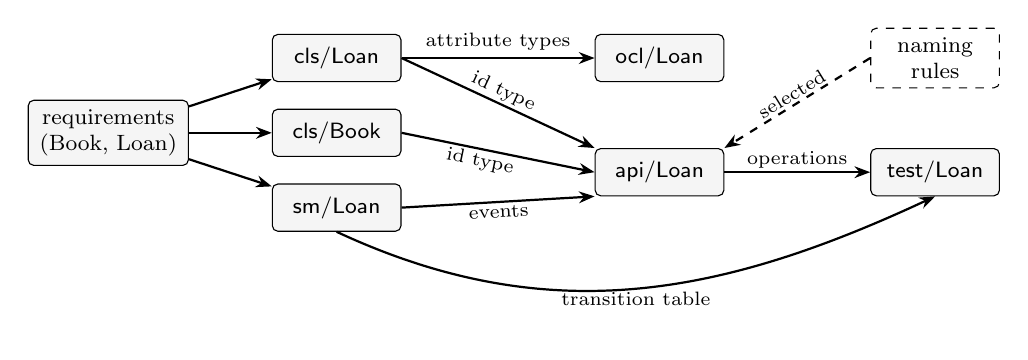
\begin{tikzpicture}[font=\footnotesize]
\node[box,text width=18mm] (r) at (0,0.2) {requirements\\(Book, Loan)};
\node[box,text width=14mm] (cl) at (2.9,1.15) {\vw{cls/Loan}};
\node[box,text width=14mm] (cb) at (2.9,0.2) {\vw{cls/Book}};
\node[box,text width=14mm] (sm) at (2.9,-0.75) {\vw{sm/Loan}};
\node[box,text width=14mm] (ol) at (7.0,1.15) {\vw{ocl/Loan}};
\node[box,text width=14mm] (api) at (7.0,-0.3) {\vw{api/Loan}};
\node[box,text width=14mm] (t) at (10.5,-0.3) {\vw{test/Loan}};
\node[box,text width=14mm,fill=white,dashed] (c) at (10.5,1.15) {naming rules};
\draw[arr] (r)--(cl); \draw[arr] (r)--(cb); \draw[arr] (r)--(sm);
\draw[arr] (cl)--node[lab,above=0.5mm,fill=none]{attribute types}(ol);
\draw[arr] (cl.east)--node[lab,above,sloped,pos=0.5,fill=none]{id type}(api.north west);
\draw[arr] (cb.east)--node[lab,below,sloped,pos=0.42,fill=none]{id type}(api.west);
\draw[arr] (sm.east)--node[lab,below,sloped,pos=0.5,fill=none]{events}(api.south west);
\draw[arr] (api)--node[lab,above,fill=none]{operations}(t);
\draw[arr] (sm.south) to[out=-25,in=-155] node[lab,below,fill=none]{transition table}(t.south);
\draw[arr,dashed] (c.west)--node[lab,above,sloped,fill=none]{selected}(api.north east);
\end{tikzpicture}
\caption{Running example: the Loan slice of the case study of Section~\ref{sec:case}. Arrows are read dependencies, labelled with the \emph{projection} of the source view that is read; the dashed arrow is shared context selected for the interface.}\label{fig:example}
\end{figure}

Figure~\ref{fig:example} shows a slice of the library model of Section~\ref{sec:case}. Agents propose the class views \vw{cls/Book} and \vw{cls/Loan}, the OCL invariants \vw{ocl/Loan}, the state machine \vw{sm/Loan} (a complete transition table of the loan lifecycle), the service interface \vw{api/Loan} and acceptance tests \vw{test/Loan}. Views read only parts of other views: the interface reads the identifier types of the class views and the event set of the state machine, and the tests read the transition table and the operation names. Table~\ref{tab:hazards} lists six hazards that no check of an individual view detects, each with the mechanism of Section~\ref{sec:approach} that removes it and the result that shows it. We refer to them as H1--H6 throughout.

\begin{table}[!ht]
\caption{Hazards of the running example, the mechanism that removes each one, and where this is shown. H4--H6 involve no change of input data.}\label{tab:hazards}
\footnotesize\setlength{\tabcolsep}{3pt}
\begin{tabular}{@{}lP{19mm}P{43mm}P{30mm}P{21mm}@{}}\toprule
 & Hazard & Instance in the Loan slice & Mechanism & Shown by\\\midrule
H1 & stale reply & a request for \vw{sm/Loan} is sent; the lifecycle changes; the old reply arrives and passes the old validator & request key with cancellation and recheck & Thm.~\ref{thm:safety} (S4), Thm.~\ref{thm:necessity}\\
H2 & stale input & \vw{api/Loan} is dispatched on the old \vw{cls/Book} while \vw{cls/Book} is regenerated & upstream gate & Thm.~\ref{thm:single}, Prop.~\ref{prop:eager}\\
H3 & global conflict & \vw{cls/Loan} types \texttt{bookId} as \texttt{Integer}, \vw{cls/Book} types \texttt{id} as \texttt{String}; each is valid alone & release barrier with $G$ & Thm.~\ref{thm:safety} (S5)\\
H4 & contract change & the OCL contract now requires named invariants & contract in the key & Thm.~\ref{thm:necessity}, RQ1\\
H5 & context change & a naming rule for interfaces is added to the shared context & selected context in the key & Thm.~\ref{thm:necessity}, RQ1\\
H6 & responsibility change & the agent that produced \vw{sm/Loan} is revoked & owner in the key; authorization & Thm.~\ref{thm:safety} (S2), RQ1\\\bottomrule
\end{tabular}
\end{table}

\subsection{Formal Preliminaries}
A \emph{labelled transition system} $(\mathcal S,\mathcal S_0,\Lambda,\to)$ has states, initial states, labels and a transition relation; runs and reachability are as usual. A predicate is an \emph{inductive invariant} if it holds initially and is preserved by every transition. For LTSs $\mathcal C,\mathcal A$ and $\alpha:\mathcal S_{\mathcal C}\to\mathcal S_{\mathcal A}$, $\mathcal C$ \emph{refines} $\mathcal A$ under $\alpha$ with stuttering if the $\alpha$-image of every run of $\mathcal C$, after removing consecutive repetitions, is a run of $\mathcal A$. A sufficient condition is a \emph{forward simulation}: $\alpha$ maps initial states to initial states, and every transition $S\to S'$ from a reachable state satisfies $\alpha(S)=\alpha(S')$ or $\alpha(S)\to\alpha(S')$~\cite{abadi1991refinement,lynch1995simulations}. \tla{}~\cite{lamport2002specifying} specifies systems as temporal formulas; the model checker TLC~\cite{yu1999tlc} checks invariants and refinement on finite instances, and the proof system TLAPS~\cite{cousineau2012tlaps} checks proofs for all instances.

% =====================================================================
\section{The Approach}\label{sec:approach}

\subsection{Overview}\label{sec:overview}
\begin{figure}[t]
\centering
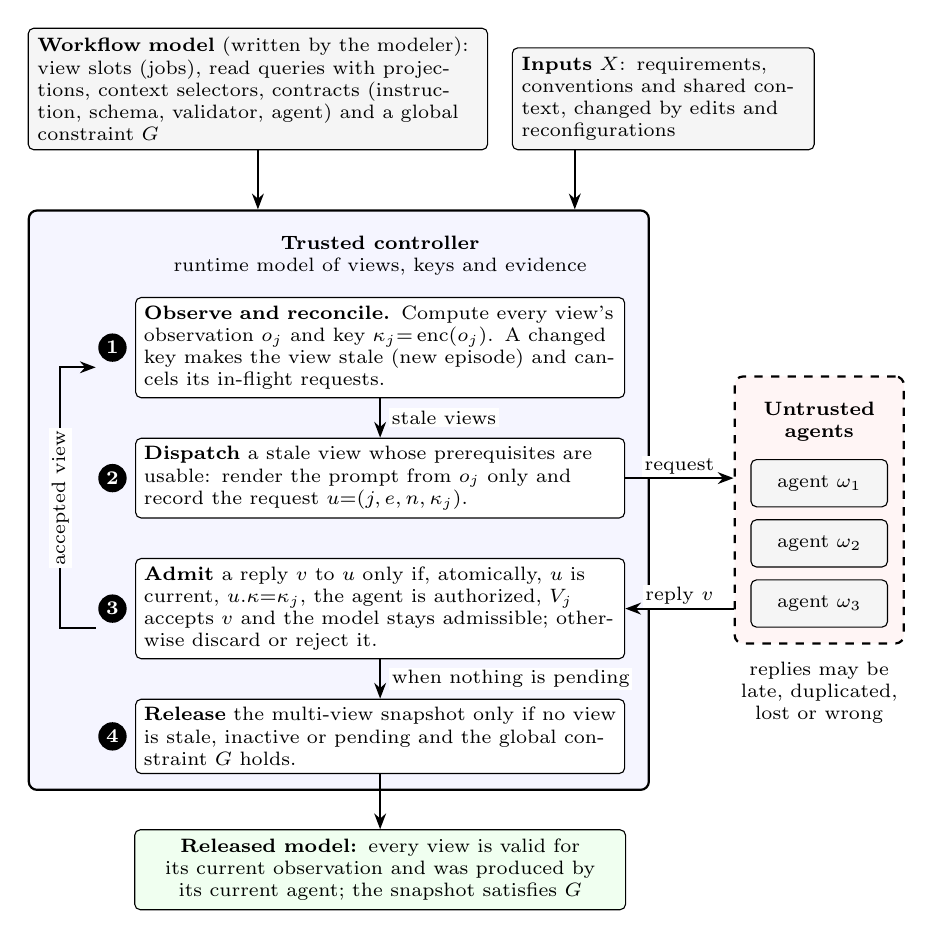
\begin{tikzpicture}[font=\scriptsize,node distance=5mm]
\node[stepbox] (s1) {\textbf{Observe and reconcile.} Compute every view's observation $o_j$ and key ${\key_j{=}\enc(o_j)}$. A changed key makes the view stale (new episode) and cancels its in-flight requests.};
\node[stepbox,below=of s1] (s2) {\textbf{Dispatch} a stale view whose prerequisites are usable: render the prompt from $o_j$ only and record the request ${u{=}(j,e,n,\key_j)}$.};
\node[stepbox,below=of s2] (s3) {\textbf{Admit} a reply $v$ to $u$ only if, atomically, $u$ is current, ${u.\key{=}\key_j}$, the agent is authorized, $V_j$ accepts $v$ and the model stays admissible; otherwise discard or reject it.};
\node[stepbox,below=of s3] (s4) {\textbf{Release} the multi-view snapshot only if no view is stale, inactive or pending and the global constraint $G$ holds.};
\foreach \s/\n in {s1/1,s2/2,s3/3,s4/4} \node[num,anchor=east] at ($(\s.west)+(-0.1,0)$) {\n};
\node[font=\scriptsize,above=1.5mm of s1,align=center] (ttl) {\textbf{Trusted controller}\\runtime model of views, keys and evidence};
\coordinate (lft) at ($(s1.west)+(-1.25,0)$);
\coordinate (rgt) at ($(s1.east)+(0.2,0)$);
\begin{scope}[on background layer]
\node[draw,thick,rounded corners=3pt,fill=blue!4,fit=(ttl)(s1)(s4)(lft)(rgt),inner xsep=1mm,inner ysep=2mm] (ctl) {};
\end{scope}
\node[box,font=\scriptsize,text width=56mm,align=left,anchor=south west] (wm) at ($(ctl.north west)+(0,0.75)$)
  {\textbf{Workflow model} (written by the modeler): view slots (jobs), read queries with projections, context selectors, contracts (instruction, schema, validator, agent) and a global constraint $G$};
\coordinate (mid) at ($(s2.east)!0.5!(s3.east)$);
\node[box,text width=15mm,font=\scriptsize] (a2) at ($(mid -| ctl.east)+(2.15,0)$) {agent $\omega_2$};
\node[box,text width=15mm,font=\scriptsize,above=1.5mm of a2] (a1) {agent $\omega_1$};
\node[box,text width=15mm,font=\scriptsize,below=1.5mm of a2] (a3) {agent $\omega_3$};
\node[font=\scriptsize\bfseries,above=1mm of a1,align=center] (agt) {Untrusted\\agents};
\begin{scope}[on background layer]
\node[draw,thick,dashed,rounded corners=3pt,fill=red!4,fit=(agt)(a1)(a3),inner sep=2mm] (ag) {};
\end{scope}
\node[font=\scriptsize,align=center,below=1mm of ag] {replies may be\\late, duplicated,\\lost or wrong};
\node[box,font=\scriptsize,text width=36mm,align=left,anchor=south west] (in) at ($(wm.south east)+(0.3,0)$)
  {\textbf{Inputs $X$}: requirements, conventions and shared context, changed by edits and reconfigurations};
\coordinate (inx) at ($(in.south west)+(0.8,0)$);
\draw[arr] (wm.south) -- (wm.south |- ctl.north);
\draw[arr] (inx) -- (inx |- ctl.north);
\node[box,font=\scriptsize,text width=60mm,fill=green!6,below=7mm of s4] (out) {\textbf{Released model:} every view is valid for its current observation and was produced by its current agent; the snapshot satisfies $G$};
\draw[arr] (s1) -- node[lab,right=1mm]{stale views} (s2);
\draw[arr] (s2.east) -- node[lab,above]{request} (s2.east -| ag.west);
\draw[arr] (s3.east -| ag.west) -- node[lab,above]{reply $v$} (s3.east);
\draw[arr] (s3) -- node[lab,right=1mm]{when nothing is pending} (s4);
\draw[arr] (s4) -- (out);
\draw[arr] ($(s3.west)+(-0.5,-0.25)$) -- ++(-0.45,0) |- node[lab,pos=0.25,rotate=90]{accepted view} ($(s1.west)+(-0.5,-0.25)$);
\end{tikzpicture}
\caption{Overview of the approach. The modeling team supplies a workflow model and the authoritative inputs (top). The trusted controller repeats four steps (1--4) and exchanges requests and replies with untrusted agents (right). An accepted view changes the observations of its consumers, which closes the loop from step~3 to step~1.}\label{fig:overview}
\end{figure}

Figure~\ref{fig:overview} summarizes the approach. The modeling team supplies two artifacts. The \emph{workflow model} is written once: it declares the view slots (\emph{jobs}) of the system model and, for each slot, what an agent may read, which shared context is selected for it and the contract under which proposals are judged, together with a global inter-view constraint $G$. The \emph{authoritative inputs} $X$ are the requirements, modeling conventions and shared context; they change over time. Agents never write the model directly. They answer requests, and the controller decides which answers become part of the model.

The central notion is the \emph{observation} $o_j$ of a view $j$: everything that determines the question the view answers, namely the data it reads (including projections of other views), the context selected for it and its contract (instruction, schema, validator, responsible agent). The controller stores the \emph{key} $\key_j=\enc(o_j)$, an injective encoding, with every request it sends and with every view it accepts. A view is \emph{usable} when the key under which it was validated equals the current key and all its prerequisites are usable. The controller then repeats four steps.
\begin{enumerate}
\item \emph{Observe and reconcile.} After every change and every acceptance, recompute the keys. A view whose key changed is \emph{stale}; it starts a new \emph{episode}, a period during which its question is fixed, and its in-flight requests are cancelled. This handles H4--H6: a new contract, a new matching naming rule or a new owner changes the key even though no data changed.
\item \emph{Dispatch} a stale view whose prerequisites are usable. The prompt is rendered from $o_j$ only, and the request records its job, episode, attempt number and key. Waiting for usable prerequisites (the \emph{upstream gate}) handles H2.
\item \emph{Admit} a reply only if, in one atomic step, the request is still current, its key equals the view's current key, the agent is still authorized, the validator accepts the view and the model remains structurally admissible. A late or duplicate reply fails the first two conditions and is discarded (H1); a reply the validator rejects consumes one attempt of a per-episode budget.
\item \emph{Release} a snapshot only when no view is stale, inactive or pending and $G$ holds on the snapshot (H3).
\end{enumerate}
Accepting a view changes the observations of the views that read it, which returns to step~1. Because observations contain projections, a regenerated view invalidates a consumer only if the part the consumer reads changed; if it did not, the consumer keeps its view (\emph{early cutoff}).

\paragraph{The life of a change.} Table~\ref{tab:trace} follows change E3 of the case study, which restricts renewal of a loan to once, through the Loan slice. The edit changes the observation of \vw{sm/Loan}, which starts a new episode; under the gate, its consumers \vw{api/Loan} and \vw{test/Loan} become inactive. When the new state machine is accepted, \vw{api/Loan} becomes active again with an \emph{unchanged} key, because it reads only the event set, which E3 does not change, so it is usable without a request. \vw{test/Loan} reads the transition table, so its key changed and it is regenerated. A duplicate of the reply to $u_1$ arrives after $u_1$ was answered and is discarded. Had E3 arrived while a request for \vw{sm/Loan} was in flight, that request would have been cancelled at step~1 and its late reply discarded in the same way. A pipeline that simply re-runs agents would instead install the late reply, which is valid for the old lifecycle (hazard H1). In contrast, change E4 (new OCL contract) changes no data. A data-only key of \vw{ocl/Loan} is unchanged, so the view stays usable and the next release contains invariants the current contract rejects; the observation-relative key changes because the contract is part of the observation.

\begin{table}[!ht]
\caption{Change E3 through the Loan slice (classes and OCL are unaffected and omitted). U: usable; S: stale; I: inactive (a prerequisite is not usable); $P$: pending requests.}\label{tab:trace}
\footnotesize\setlength{\tabcolsep}{3pt}
\begin{tabular}{@{}rP{27mm}P{28mm}P{24mm}P{22mm}l@{}}\toprule
 & Transition & \vw{sm/Loan} & \vw{api/Loan} & \vw{test/Loan} & $P$\\\midrule
0 & (released model) & U & U & U & $\emptyset$\\
1 & $\mathsf{Edit}$(E3) & S, new episode, new key & I & I & $\emptyset$\\
2 & $\Disp$(\vw{sm/Loan}) & S, request $u_1$ & I & I & $\{u_1\}$\\
3 & $\Acc(u_1,v)$ & U & U, key unchanged (early cutoff) & S, new key & $\emptyset$\\
4 & duplicate reply to $u_1$ & discarded ($u_1\notin P$) & U & S & $\emptyset$\\
5 & $\Disp$(\vw{test/Loan}) & U & U & S, request $u_2$ & $\{u_2\}$\\
6 & $\Acc(u_2,v')$ & U & U & U & $\emptyset$\\
7 & $\mathsf{Publish}$ & \multicolumn{4}{l}{snapshot released if $G$ holds}\\\bottomrule
\end{tabular}
\end{table}

The remainder of this section makes these steps precise: the workflow metamodel (Section~\ref{sec:metamodel}), observations and keys (Section~\ref{sec:obs}), the controller state (Section~\ref{sec:state}) and its transitions (Section~\ref{sec:rules}).

\subsection{Workflow Models}\label{sec:metamodel}
\begin{figure}[!ht]
\centering
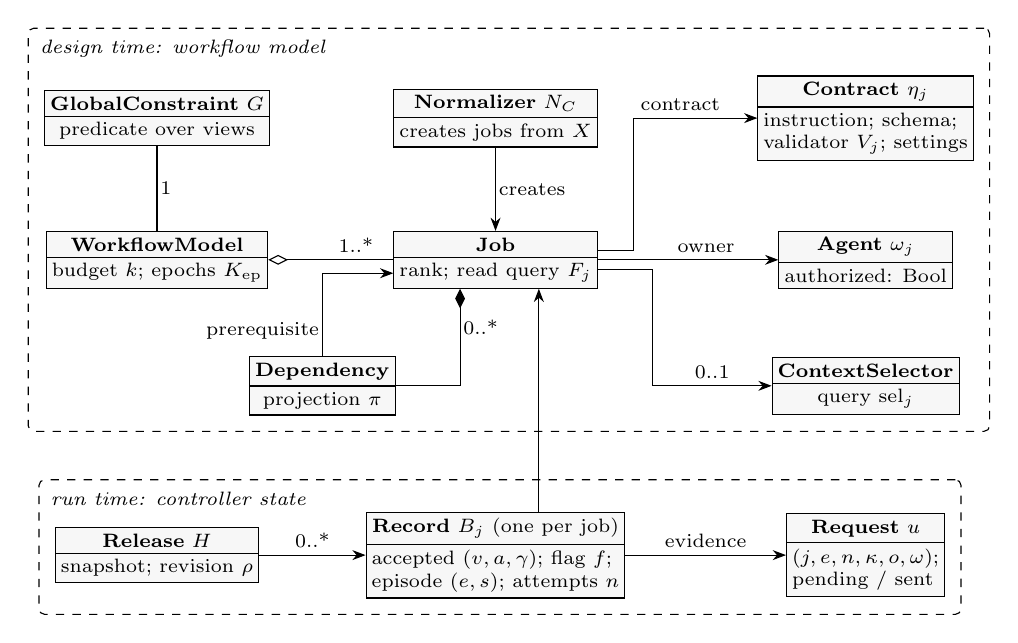
\begin{tikzpicture}[font=\scriptsize]
\node[cls] (g)   at (0,1.8)    {\textbf{GlobalConstraint} $G$\nodepart{second}predicate over views};
\node[cls] (wf)  at (0,0)      {\textbf{WorkflowModel}\nodepart{second}budget $k$; epochs $K_{\mathrm{ep}}$};
\node[cls] (n)   at (4.3,1.8)  {\textbf{Normalizer} $N_C$\nodepart{second}creates jobs from $X$};
\node[cls] (job) at (4.3,0)    {\textbf{Job}\nodepart{second}rank; read query $F_j$};
\node[cls] (dep) at (2.1,-1.6){\textbf{Dependency}\nodepart{second}projection $\pi$};
\node[cls] (ct)  at (9.0,1.8)  {\textbf{Contract} $\eta_j$\nodepart{second}instruction; schema;\\validator $V_j$; settings};
\node[cls] (ag)  at (9.0,0)    {\textbf{Agent} $\omega_j$\nodepart{second}authorized: Bool};
\node[cls] (sel) at (9.0,-1.6) {\textbf{ContextSelector}\nodepart{second}query $\operatorname{sel}_j$};
\draw[{Diamond[open,length=2.5mm]}-] (wf.east)--node[lab,above=0.5mm,pos=0.7]{1..*}(job.west);
\draw[-] (g.south)--node[lab,right]{1}(wf.north);
\draw[-{Stealth}] (n.south)--node[lab,right]{creates}(job.north);
\coordinate (b) at ($(job.east)+(0.45,0)$);
\draw[-{Stealth}] ($(job.east)+(0,0.12)$) -| ($(b)+(0,0.12)$) |- (ct.west);
\node[lab,above=0.5mm] at ($(b |- ct.west)!0.38!(ct.west)$) {contract};
\draw[-{Stealth}] (job.east)--node[lab,pos=0.6,above=0.5mm]{owner}(ag.west);
\draw[-{Stealth}] ($(job.east)+(0,-0.12)$) -| ($(b)+(0.25,-0.12)$) |- (sel.west);
\coordinate (b2) at ($(b)+(0.25,0)$);
\node[lab,above=0.5mm] at ($(b2 |- sel.west)!0.5!(sel.west)$) {0..1};
\draw[{Diamond[length=2.5mm]}-] ($(job.south)+(-0.45,0)$) |- node[lab,pos=0.2,right]{0..*}(dep.east);
\draw[-{Stealth}] (dep.north) |- node[lab,pos=0.15,left]{prerequisite}($(job.west)+(0,-0.17)$);
\node[cls] (rec) at (4.3,-3.75) {\textbf{Record} $B_j$ (one per job)\nodepart{second}accepted $(v,a,\gamma)$; flag $f$;\\episode $(e,s)$; attempts $n$};
\node[cls] (req) at (9.0,-3.75) {\textbf{Request} $u$\nodepart{second}$(j,e,n,\key,o,\omega)$;\\pending / sent};
\node[cls] (rel) at (0,-3.75)   {\textbf{Release} $H$\nodepart{second}snapshot; revision $\rho$};
\draw[-{Stealth}] ($(rec.north)+(0.55,0)$) -- ($(job.south)+(0.55,0)$);
\draw[-{Stealth}] (rec.east) -- node[lab,above=0.5mm]{evidence}(req.west);
\draw[-{Stealth}] (rel.east) -- node[lab,above=0.5mm]{0..*}(rec.west);
\coordinate (t1) at ($(ct.north)+(0,0.4)$);
\coordinate (t2) at ($(rel.north)+(0,0.4)$);
\begin{scope}[on background layer]
\node[draw,dashed,rounded corners=2pt,fit=(t1)(g)(sel)(ct)(dep),inner sep=2mm,label={[font=\scriptsize\itshape,anchor=north west,inner sep=1.5mm]north west:design time: workflow model}] {};
\node[draw,dashed,rounded corners=2pt,fit=(t2)(rel)(rec)(req),inner sep=2mm,label={[font=\scriptsize\itshape,anchor=north west,inner sep=1.5mm]north west:run time: controller state}] {};
\end{scope}
\end{tikzpicture}
\caption{Coordination metamodel (simplified). Design time: a workflow model and its jobs; inputs and shared context are not shown. Run time: the controller state, a runtime model with one record per job, the requests it sent and its releases.}\label{fig:metamodel}
\end{figure}

Figure~\ref{fig:metamodel} shows the metamodel. At design time, a \emph{workflow model} contains jobs, each a slot for one view element that an agent may fill. A job has a rank, a \emph{read query} $F_j$ over the authoritative inputs, \emph{dependencies} on other jobs, each with a \emph{projection} $\pi$ of the prerequisite's value, an optional context selector, a responsible agent and a \emph{contract} that names the instruction, output schema, validator, its execution environment and the generation settings. A \emph{structural normalizer} $N_C$ instantiates jobs from the inputs (one class view per entity, one state machine per entity with a lifecycle), and a \emph{global constraint} $G$ expresses inter-view consistency. At run time, the controller state holds one \emph{record} per job, the \emph{requests} it sent and its \emph{releases}; Section~\ref{sec:state} defines them.

Figure~\ref{fig:workflow} shows the workflow model of the case study in a compact textual notation. Each \texttt{job} declaration maps one-to-one onto a job declaration of our implementation, which states the same fields in Python (Section~\ref{sec:case}). The declaration is what a modeler writes; everything else in this article is supplied once by the controller. It makes the hazards of Table~\ref{tab:hazards} explicit: the contract of \vw{ocl/E} is named (H4), the interface selects naming rules (H5), the owner of every job is named (H6), and the projections state that \vw{api/E} reads only identifier types and events (Table~\ref{tab:trace}, step~3).

\begin{figure}[!ht]
\centering
\begin{minipage}{0.97\textwidth}
\footnotesize
\begin{verbatim}
workflow Library   budget 4   feedback-epochs 1
  global G: every reference attribute has the identifier type of its target class
  for E in Entities:
    job cls/E   rank 1  owner A  contract cls-v1
        reads  req[E].text, req[E].attributes, conventions
  for E in Entities with invariants:
    job ocl/E   rank 2  owner A  contract ocl-v1
        reads  req[E].constraints
        dep    cls/E                    project attributes
  for E in Entities with lifecycle:
    job sm/E    rank 1  owner B  contract sm-v1
        reads  req[E].lifecycle
    job api/E   rank 3  owner C  contract api-v1
        dep    cls/E, cls/Book, cls/Member  project attributes.id
        dep    sm/E                     project events
        select context.rules where scope = "api"
    job test/E  rank 4  owner C  contract test-v1
        dep    sm/E                     project (initial, table)
        dep    api/E                    project operations
  contract ocl-v1: instruction "Write OCL invariants ..."  schema OclList
                   validator ocl-equivalence-on-grid  model llm  temperature 0.7
\end{verbatim}
\end{minipage}
\caption{Workflow model of the case study (contracts other than \texttt{ocl-v1} omitted). Change E4 replaces \texttt{ocl-v1} by a contract that requires named invariants; change E6 replaces owner \texttt{B}.}\label{fig:workflow}
\end{figure}

\paragraph{Well-formedness.} Workflow models must satisfy four static rules, which a modeling tool can check when the workflow model is edited. They are the assumptions W1--W4 of Table~\ref{tab:assumptions}: (W1) the prerequisite relation is a finite strict order and every read query, selector, projection, validator and structural expression of a job refers only to the inputs and to the job's prerequisites; (W2) the normalizer is deterministic, terminating and idempotent, and agents write only primitive values; (W3) every configuration change that affects a job, including a change of owner or budget, changes the job's contract identity, and contract identities are never reused; (W4) whether a job exists, and its query, selector and validator, depend only on the inputs and on values of its prerequisites. W3 makes ``the question changed'' visible in the key; W4 rules out jobs that are created or deleted by sibling views.

\subsection{Observations and Keys}\label{sec:obs}
A \emph{configuration} $C$ is an instance of the design-time metamodel: a finite set $\Jobs_C$ of \emph{potential} jobs (one per job kind and admissible entity name), a strict partial order $\prec$ on $\Jobs_C$ (\emph{prerequisites}), and for each job $j$ an owner $\omega_j$, a read function $F_j$ (including the projections of its dependencies), a context selector $\operatorname{sel}_j$, a validator $V_j$ and a contract $\eta_j$ that identifies the instruction, output schema, validator and its environment, generation settings, budget and $\omega_j$. $X$ denotes the authoritative inputs (requirements and immutable context snapshots).

All derived notions are defined together by induction on $\prec$; the definition is well founded because $\prec$ is (W1). For a state $S$ (Section~\ref{sec:state}) and a job $j$, let $Z_{\prec j}(S)$ consist of $X$ and the values of the usable prerequisites of $j$. Then $j$ \emph{exists} if $j\in N_C(X,Z_{\prec j})$, and its \emph{observation} and \emph{key} are
\begin{equation}\label{eq:obs}
o_j(S)=\bigl(F_j(Z_{\prec j}),\ \operatorname{sel}_j(Z_{\prec j}),\ \eta_j\bigr),\qquad \key_j(S)=\enc(o_j(S)),
\end{equation}
where $\enc$ is a canonical injective encoding. If required context is unavailable, $o_j=\nodata$. $F_j$ and $\operatorname{sel}_j$ are queries (``the identifier type of \vw{cls/Book}'', ``all naming rules for interfaces''), so membership is observable: adding a matching rule changes $o_j$, whereas a change of \vw{cls/Book} that leaves its identifier type unchanged does not.

\begin{definition}[Adequacy and soundness]\label{def:adequate}
Let $R_j(Z,v)$ be the intended relation for job $j$, e.g.\ ``$v$ is a test suite that exercises the current loan lifecycle''. The observation is \emph{adequate} for $R_j$ if there is $\widehat R_j$ with $R_j(Z,v)\iff\widehat R_j(o_j(Z),v)$ for all admissible $Z,v$; a validator is \emph{sound} if $V_j(o,v)\Rightarrow\widehat R_j(o,v)$. $G$ is sound for a relation $R_G$ over snapshots if $G$ implies $R_G$.
\end{definition}
An observation of \vw{test/Loan} that contained the operation names but not the transition table would not be adequate: models with equal interfaces and different lifecycles require different tests.

\subsection{Controller State}\label{sec:state}
A state is $S=(C,X,B,P,\Sent,H,\nu,\rho)$. For each job, the \emph{record} $B_j=(\mathit{acc},f,e,s,n)$ holds an accepted triple $\mathit{acc}=(v,a,\gamma)$ of value, \emph{validated key} and evidence (the producing request), or $\bot$; a failure flag $f$; an episode nonce $e$ with \emph{episode key} $s$, the key the current episode was started for; and an attempt counter $n\in\{0,\ldots,k\}$ for the budget $k\ge1$. $P$ is the set of pending requests and $\Sent\supseteq P$ the append-only set of all sent ones. A request $u=(j,e,n,\key,o,\omega)$ records its job, episode, attempt, key, observation and owner; its identity is $(j,e,n)$. $H$ is the last release, $\nu$ a nonce counter and $\rho$ a revision counter. Three keys thus appear per job: the current key $\key_j(S)$, the episode key $s_j$ and the validated key $a$.

A job is \emph{active} if it exists, $o_j\neq\nodata$, its owner is authorized and all its prerequisites are usable. Then
\begin{align}
\fresh_j(S)&\iff B_j.\mathit{acc}=(v,a,\gamma)\land a=\key_j(S),\label{eq:fresh}\\
U_j(S)&\iff \Act_j(S)\land\fresh_j(S),\quad\text{where }\Act_j(S)\text{ includes }\textstyle\bigwedge_{i\prec j}U_i(S),\label{eq:usable}\\
\Stale(S)&=\{j:\Act_j(S)\land\neg U_j(S)\},\qquad \Inact(S)=\{j:j\text{ exists}\land\neg\Act_j(S)\}.\label{eq:obl}
\end{align}
A job is \emph{usable} ($U_j$), \emph{stale} or \emph{inactive}; inactive jobs are suspended (context unavailable), unauthorized or waiting for a prerequisite. Equation~\eqref{eq:usable} is the \emph{upstream gate}: consumers never read a view computed over stale inputs.

\subsection{Reconciliation and Transitions}\label{sec:recon}\label{sec:rules}
After every committed edit, reconfiguration or acceptance, the reconciliation operator $\mathcal R$ normalizes the candidate state $S'$ in $\prec$-order and, for each job $j$ active in $S'$, sets
\begin{equation}\label{eq:recon}
B'_j=\begin{cases}B_j&\text{if }j\text{ was active in }S\text{ and }s_j=\key_j(S'),\\(B_j.\mathit{acc},\ \mathit{false},\ \nu',\ \key_j(S'),\ 0)&\text{otherwise (new episode)},\end{cases}
\end{equation}
where $\nu'$ is a fresh nonce drawn by incrementing $\nu$. It then \emph{cancels} every request in $P$ whose job is inactive or whose episode, key or owner differs from the job's current one. A new episode retains the accepted triple; by~\eqref{eq:fresh} it is usable again at once if its validated key equals the new key (\emph{early cutoff}, step~3 of Table~\ref{tab:trace}). A discarded candidate discards its nonces, so request identities are never reused, and every $u\in\Sent$ satisfies $u.e\le\nu$.

Table~\ref{tab:rules} lists the transitions, each one atomic transaction. The environment is fully nondeterministic: any value may be delivered for any request in $\Sent$, any number of times, or never. This over-approximates every agent behavior without probabilistic assumptions. The \emph{commit guard} of $\Acc$ contains two defenses against obsolete replies: \emph{cancellation} (only $u\in P$ is considered, and $\mathcal R$ removes obsolete requests) and the \emph{recheck} $u.e=e_j\land u.\key=\key_j(S)$. Validation may run outside the transaction on the immutable $u.o$ if the guard is rechecked inside it, as in OCC~\cite{occ}. Release requires
\begin{equation}\label{eq:pub}
\Pub(S)\iff \Inact(S)=\emptyset\land \Stale(S)=\emptyset\land P=\emptyset\land G(S)
\end{equation}
and installs exactly the snapshot it tested.

\begin{table}[!ht]
\caption{Controller transitions and the abstract action of $\mathcal A$ (Section~\ref{sec:refine}) each maps to under $\alpha$. Unmentioned components are unchanged. \emph{Admissible}: the structural expressions of every configured consumer hold on the candidate (Section~\ref{sec:deferred}).}\label{tab:rules}
\footnotesize\setlength{\tabcolsep}{3pt}
\begin{tabular}{@{}P{16mm}P{50mm}P{44mm}P{11mm}@{}}\toprule
Transition & Guard & Effect & Abstract\\\midrule
$\mathsf{Edit}(\delta)$ & authorized input change; candidate admissible & install $\delta$; $\mathcal R$; $\rho{+}{+}$ & Edit\\
$\mathsf{Reconf}(C')$ & $C'$ satisfies W1--W3, R2 & install $C'$; $\mathcal R$; $\rho{+}{+}$ & Edit\\
$\Disp(j)$ & $j\in\Stale(S)$; $\neg f_j$; $n_j<k$; no $u\in P$ for $j$ & $n_j{+}{+}$; add $u=(j,e_j,n_j,\key_j,o_j,\omega_j)$ to $P$ and $\Sent$ & Attempt\\
$\Acc(u,v)$ & (1) $u\in P$; (2) $u.e=e_j$ and $u.\key=\key_j(S)$; (3) $\omega_j$ authorized; (4) $V_j(u.o,v)$; (5) candidate admissible & $\mathit{acc}_j\gets(v,u.\key,u)$; $f_j\gets\mathit{false}$; remove $u$; $\mathcal R$; $\rho{+}{+}$ & Accept\\
$\mathsf{Reject}(u)$, $\mathsf{Timeout}(u)$ & (1)--(3) hold; (4) or (5) fails, or timeout & remove $u$; $f_j\gets(n_j=k)$ & Fail\\
$\mathsf{Discard}(u)$ & $u\in\Sent$ and (1) or (2) fails & remove $u$ from $P$ if present & stutter\\
$\mathsf{Publish}$ & $\Pub(S)$, Eq.~\eqref{eq:pub} & $H\gets(\text{snapshot},\rho)$ & Publish\\\bottomrule
\end{tabular}
\end{table}

\subsection{Deferred Structural Checks}\label{sec:deferred}
A generated value may be read by a structural expression of a later job's normalization. In the running example, the identifier type proposed for \vw{cls/Book} determines the type of the \texttt{bookId} parameter of \vw{api/Loan}, which the interface schema may require to be a string. If \vw{api/Loan} is not yet enabled when \vw{cls/Book} is accepted with \texttt{Integer}, a natural design checks nothing and later refuses the edit that enables the interface; Proposition~\ref{prop:hazard} shows that this can block a revision forever. We adopt two rules. (a) \emph{Configured-consumer checks}: $\Acc$ evaluates, on the candidate, the structural expressions of every \emph{configured} consumer of the slot, enabled or not. (b) \emph{Invalidate, do not refuse}: whenever $\mathcal R$ would make a structural expression fail because of a retained generated value (after an $\mathsf{Edit}$ or $\mathsf{Reconf}$, or when $\mathcal R$ makes a retained value usable again by early cutoff), that value is \emph{demoted}: its accepted triple is dropped, so its job becomes stale, and normalization is retried. Only failures caused by the inputs themselves reject an edit. Rule (b) terminates because each retry demotes one of finitely many values.

\begin{table}[!ht]
\caption{Assumptions and the results that use them. W: static well-formedness of workflow models (Section~\ref{sec:metamodel}); R: runtime; E: environment; D: domain.}\label{tab:assumptions}
\footnotesize\setlength{\tabcolsep}{4pt}
\begin{tabular}{@{}lP{88mm}P{26mm}@{}}\toprule
ID & Assumption & Used by\\\midrule
W1 & $\prec$ is a finite strict order; $F_j$, $\operatorname{sel}_j$, $V_j$, projections and structural expressions read only $X$ and values of prerequisites of $j$ & all\\
W2 & $N_C$ deterministic, terminating, idempotent; agents write primitive slots only; rules (a), (b) & Thm.~\ref{thm:safety}, \ref{thm:single}, \ref{thm:termination}, Lem.~\ref{lem:react}\\
W3 & $\enc$ injective; every configuration change that affects $j$ (owner, budget, validator, \ldots) changes $\eta_j$; contract identities are never reused & Lem.~\ref{lem:currency}, \ref{lem:local}, Thm.~\ref{thm:safety}--\ref{thm:reconfig}\\
W4 & existence, $F_j$, $\operatorname{sel}_j$ and $V_j$ of $j$ depend only on $X$ and values of prerequisites of $j$ & Thm.~\ref{thm:single}, \ref{thm:termination}\\
R1 & transitions are linearizable; recorded requests are immutable & Lem.~\ref{lem:currency}, Thm.~\ref{thm:safety}, \ref{thm:refinement}\\
R2 & validators are total and deterministic on observations & Thm.~\ref{thm:safety}\\
E1 & inputs and configuration eventually stop changing; the controller is fair; every request is eventually resolved or timed out & Thm.~\ref{thm:termination}\\
D1 & observations adequate; validators and $G$ sound & Cor.~\ref{cor:domain}\\\bottomrule
\end{tabular}
\end{table}

% =====================================================================
\section{Safety, Refinement and Necessity}\label{sec:safety}
This section answers the question a modeler asks first: what can be trusted about a released model, whatever the agents do? The answer is Theorem~\ref{thm:safety}: every usable view is valid for its current observation and every release passed the barrier. Theorem~\ref{thm:refinement} lets a modeler reason about the workflow model as if requests were instantaneous, and Theorem~\ref{thm:necessity} shows that no defense can be dropped.

\subsection{Request Currency and Safety}
Most results rest on one invariant: the controller never holds a request that answers a question other than the current one.

\begin{lemma}[Request currency]\label{lem:currency}
Under W1--W3 and R1, every reachable state satisfies: (0) every active job $j$ has $s_j=\key_j(S)$, and every $u\in\Sent$ has $u.e\le\nu$; and for every $u\in P$ with job $j$: (i) $j$ is active; (ii) $u.e=e_j$, $u.\key=s_j=\key_j(S)$ and $u.\omega=\omega_j$; (iii) $\neg\fresh_j(S)$; (iv) no other request in $P$ has job $j$; (v) $1\le u.n\le n_j$.
\end{lemma}
\begin{proof}
Initially $P=\Sent=\emptyset$ and $\mathcal R$ has set $s_j=\key_j$ for every active job. $\Disp$, $\mathsf{Reject}$, $\mathsf{Timeout}$, $\mathsf{Discard}$ and $\mathsf{Publish}$ change neither $C$, $X$ nor any accepted triple, hence no observation, key or activity, so (0) is preserved. $\Disp(j)$ adds $u$ only if $j\in\Stale(S)$, so $j$ is active and not fresh; it records the current $e_j$, $\key_j=s_j$ (by (0)) and $\omega_j$, and $u.n=n_j\ge1$ after the increment; (iv) holds by its guard. The other four of these transitions only remove requests or set $f_j$. $\mathsf{Edit}$, $\mathsf{Reconf}$ and $\Acc$ end with $\mathcal R$, which establishes (0) by~\eqref{eq:recon}, and $\Acc(u,v)$ removes $u$ itself. For a remaining $u'\in P$ with job $i$: if $i$ becomes inactive or its key, episode or owner changes, $\mathcal R$ cancels $u'$. Otherwise $i$ stays active with key $s_i=u'.\key$ and, by~\eqref{eq:recon}, an unchanged record; since $i$ was not fresh for this key before and its triple is unchanged, it is not fresh now, and $n_i$ is unchanged.
\end{proof}

By Lemma~\ref{lem:currency}(iii), $P\ne\emptyset$ implies $\Stale(S)\ne\emptyset$, so the conjunct $P=\emptyset$ in~\eqref{eq:pub} is implied; we keep it as a defense that remains valid if cancellation is disabled.

\begin{theorem}[Observation-relative safety]\label{thm:safety}
Under W1--W3, R1 and R2, every reachable state satisfies:
(S1) the installed structure is admissible for every configured consumer;
(S2) every accepted triple $(v,a,\gamma)$ has $\gamma\in\Sent$, $\gamma.\key=a$, $V(\gamma.o,v)$ for the validator of $\gamma$'s contract, and an owner authorized at acceptance;
(S3) every usable value is valid for the current observation: $U_j(S)\Rightarrow V_j(o_j(S),v_j)$;
(S4) every accepted reply was current and authorized at its linearization point;
(S5) every installed release $H$ was, when installed, a snapshot in which every existing job was usable, no request was pending and $G$ held;
(S6) for every job $j$ and episode $e$, $|\{u\in\Sent:u.j=j,u.e=e\}|\le k$, with equality to $n_j$ for $e=e_j$.
\end{theorem}
\begin{proof}
We show that (S1)--(S6) together with Lemma~\ref{lem:currency} are inductive. Initially no value is accepted, $\Sent=\emptyset$, and the structure is the normal form of $X$, admissible by W2.
(S1) $\Acc$ installs a candidate only if it is admissible for all configured consumers (rule (a)); $\mathsf{Edit}$, $\mathsf{Reconf}$ and reactivations in $\mathcal R$ install only admissible candidates, demoting offending values by rule (b); other transitions leave structure unchanged.
(S2) Only $\Acc(u,v)$ creates a triple, namely $(v,u.\key,u)$ with $u\in\Sent$; its guard requires $V_j(u.o,v)$ and authorization of $\omega_j=u.\omega$. Triples are never modified; they are retained or, by rule (b), dropped.
(S4) At the linearization point of $\Acc(u,v)$ the recheck gives $u.e=e_j$ and $u.\key=\key_j(S)$, and the guard gives authorization.
(S3) Let $U_j(S)$ with $\mathit{acc}_j=(v,a,\gamma)$. By~\eqref{eq:fresh}, $a=\key_j(S)$; by (S2), $\gamma.\key=a$ and $V(\gamma.o,v)$. $\Disp$ records $\gamma.\key=\enc(\gamma.o)$, and requests are immutable (R1). Hence $\enc(\gamma.o)=\enc(o_j(S))$ and, by injectivity (W3), $\gamma.o=o_j(S)$. The observation contains the contract identity, which is never reused and determines the validator (W3), so $\gamma$'s validator is the current $V_j$, and R2 gives $V_j(o_j(S),v)$.
(S5) $\mathsf{Publish}$ evaluates~\eqref{eq:pub} on an immutable snapshot and installs it (R1); $\Inact=\Stale=\emptyset$ means every existing job is usable. Later transitions do not relabel $H$.
(S6) $n_j$ grows only by $\Disp$, which requires $n_j<k$ and adds one request with episode $e_j$ to $\Sent$. A new episode resets $n_j$ to $0$ with a nonce larger than every $u.e$ in $\Sent$ (Lemma~\ref{lem:currency}(0)), so $\Sent$ holds no request of it; earlier episodes receive no new requests. A change of $k$ changes every contract (W3) and hence starts new episodes.
\end{proof}

\begin{corollary}[Validator-relative correctness]\label{cor:domain}
Under the assumptions of Theorem~\ref{thm:safety} and D1, every usable view satisfies $R_j(Z(S),v_j)$, and every released snapshot satisfies $R_G$.
\end{corollary}
\begin{proof}
(S3) gives $V_j(o_j,v_j)$; soundness gives $\widehat R_j(o_j,v_j)$; adequacy gives $R_j(Z,v_j)$. The second claim follows from (S5) and soundness of $G$.
\end{proof}
Corollary~\ref{cor:domain} separates two kinds of guarantee: Theorem~\ref{thm:safety} holds for \emph{any} validator, whereas the correctness of a view with respect to the modeler's intent is inherited from the validator and no more. For a modeling team, this places the specification effort where MDE already places it: in well-formedness rules, constraints and executable semantics of the views. For finite behavioral views, such as the state machines of the case study, a complete validator turns Theorem~\ref{thm:safety} into full functional correctness (Appendix~\ref{app:finite}).

\subsection{Refinement of an Atomic Specification}\label{sec:refine}
The abstract machine $\mathcal A$ has the same configuration, inputs, records, budgets, failure flags, nonce and revision counters and release, but no requests: request transport is erased. Its actions are listed in Table~\ref{tab:abstract}. The refinement mapping erases requests and evidence:
\begin{equation}\label{eq:alpha}
\alpha(C,X,B,P,\Sent,H,\nu,\rho)=(C,X,B^{\circ},H,\nu,\rho),
\end{equation}
where $B^{\circ}$ replaces the evidence $\gamma$ of each accepted triple by a placeholder. Because $\alpha$ keeps attempt counters, concrete $\Disp$ must map to $\mathsf{Attempt}$: mapping it to a stutter while the incremented counter stays visible would be unsound.

\begin{table}[!ht]
\caption{Actions of the atomic specification $\mathcal A$. Abstract $\mathsf{Accept}$ reads only the current observation $o_j$; in the controller it reads the observation $u.o$ recorded at dispatch.}\label{tab:abstract}
\footnotesize\setlength{\tabcolsep}{3pt}
\begin{tabular}{@{}lP{55mm}P{50mm}@{}}\toprule
Action & Guard & Effect\\\midrule
$\mathsf{Attempt}(j)$ & $j\in\Stale$; $\neg f_j$; $n_j<k$ & $n_j{+}{+}$\\
$\mathsf{Accept}(j,v)$ & $j\in\Stale$; $\omega_j$ authorized; $n_j>0$; $V_j(o_j,v)$; candidate admissible & $\mathit{acc}_j\gets(v,\key_j,\cdot)$; $f_j\gets\mathit{false}$; $\mathcal R$; $\rho{+}{+}$\\
$\mathsf{Fail}(j)$ & $j\in\Stale$; $n_j>0$ & $f_j\gets(n_j=k)$\\
$\mathsf{Edit}$ & as $\mathsf{Edit}$ or $\mathsf{Reconf}$ in Table~\ref{tab:rules} & install; $\mathcal R$; $\rho{+}{+}$\\
$\mathsf{Publish}$ & $\Inact=\Stale=\emptyset$ and $G$ & $H\gets(\text{snapshot},\rho)$\\\bottomrule
\end{tabular}
\end{table}

\begin{theorem}[Forward simulation]\label{thm:refinement}
Under W1--W3, R1 and R2, the asynchronous controller refines $\mathcal A$ under $\alpha$ with stuttering. Hence asynchronous delivery cannot produce a view or release that the atomic specification forbids.
\end{theorem}
\begin{proof}
Initial states correspond. Consider a transition from a reachable $S$. $\Disp(j)$ has the guard of $\mathsf{Attempt}(j)$ plus extra conjuncts and the same effect on $B^{\circ}$. For $\Acc(u,v)$ with job $j$: by Lemma~\ref{lem:currency}, $j$ is active and not fresh, so $j\in\Stale(S)$, and $n_j\ge u.n\ge1$; $u.\key=\key_j(S)$ and injectivity give $u.o=o_j(S)$, so $V_j(u.o,v)$ is the abstract validity guard; both machines install the same value and validated key and apply the same $\mathcal R$ with the same nonces, and $\alpha$ hides the evidence. $\mathsf{Reject}$ and $\mathsf{Timeout}$ of a current request map to $\mathsf{Fail}(j)$ by the same argument. $\mathsf{Discard}$ changes only $P$, which $\alpha$ erases. $\mathsf{Edit}$, $\mathsf{Reconf}$ and $\mathsf{Publish}$ have equal effects on the projected components, and concrete $\Pub$ implies the abstract guard. We claim neither the converse nor a liveness correspondence.
\end{proof}
For a modeler, Theorem~\ref{thm:refinement} means that the workflow model can be reviewed and simulated with the atomic semantics, in which every acceptance answers the question of the current model; late, duplicate and lost replies add no observable behavior.

\subsection{Necessity of the Defenses}\label{sec:necessity}
Theorem~\ref{thm:safety} shows that the defenses suffice; we now show that each is needed. Write $\mathcal C_{-m}$ for the controller with mechanism $m$ removed and everything else unchanged. Properties of $\mathcal C_{-m}$ are evaluated with the unablated definitions, i.e.\ against the true observation and the true usability. We write (S3$^{\uparrow}$) for the part of (S3) that the gate provides: a usable job has only usable prerequisites.

\begin{theorem}[Necessity]\label{thm:necessity}
For every row of Table~\ref{tab:necessity} there is a configuration satisfying W1--W4 with at most two jobs and a finite run of $\mathcal C_{-m}$ that violates the listed property. Removing \emph{only} cancellation or \emph{only} the recheck preserves (S3) and (S4); the two form one necessary class.
\end{theorem}
\begin{proof}
Each run in Table~\ref{tab:necessity} is a few transitions long and satisfies W1--W4 by inspection. We give the first row on the running example (hazard H1). Dispatch $u$ for \vw{sm/Loan} on observation $o_0$ (old lifecycle); apply E3, which starts a new episode with observation $o_1$; deliver a table that is valid for $o_0$. Without cancellation $u$ stays in $P$, and without the recheck nothing compares $u.\key$ with $\key_j$, so $\Acc(u,v)$ installs $(v,\enc(o_0),u)$, violating (S4): the record carries provenance from an obsolete question and displaces the retained evidence. In the contract and context rows (H4, H5) the key itself fails to change, so the obsolete value even becomes usable and (S3) fails whenever the change alters validity.
For the second claim: with the recheck but no cancellation, the guard of $\Acc$ requires $u.e=e_j$ and $u.\key=\key_j(S)$ explicitly, which is all the proofs of (S3) and (S4) use. With cancellation but no recheck, the proof of Lemma~\ref{lem:currency} uses only cancellation, so every $u\in P$ satisfies these equalities anyway.
\end{proof}

\begin{table}[!ht]
\caption{Necessity of the defenses. \emph{Evidence}: M = violated by a TLC mutant (Table~\ref{tab:tlc}), with the property in parentheses where TLC checks only part of the row; T = regression test of the executable controller; C = observed in the case study (Section~\ref{sec:case}); P = paper construction only.}\label{tab:necessity}
\footnotesize\setlength{\tabcolsep}{3pt}
\begin{tabular}{@{}P{30mm}lP{16mm}P{55mm}l@{}}\toprule
Removed mechanism & Hazard & Lost & Violating run & Ev.\\\midrule
Cancellation and recheck & H1 & S4 & dispatch on $o_0$; edit to $o_1$; deliver old valid reply & M, C\\
Contract in key & H4 & S3, S4 & dispatch; replace validator, inputs unchanged; deliver reply valid only for the old validator & M (S4), C\\
Context membership in key & H5 & S3, S4 & dispatch; add a matching rule; deliver reply that ignores it & M (S4), C\\
Owner authorization & H6 & S2, S4 & dispatch; revoke owner; deliver reply & M, C\\
Upstream gate & H2 & S3$^{\uparrow}$ & edit $j_1$'s input; dispatch $j_2$ on the old value of $j_1$; accept & C\\
Global predicate $G$ & H3 & S5 & two locally valid class views disagree on an identifier type; release & P\\
Candidate admissibility & -- & S1 & accept a locally valid integer identifier read by a string-typed identity & P\\
Budget persistence & -- & S6 & exhaust $k$ attempts; reset counter without new episode; dispatch & M\\
Suspension in $\Pub$ & -- & S5 & suspend a required job; release with no stale job & M\\
Revision check in a two-step $\Pub$ & -- & S5 & test $\Pub$ on a snapshot; edit; install the edited snapshot & M\\
Fresh request identities & H1 & S4 & delete and recreate $j$ (episode counter restarts); deliver duplicate of the old request & T\\\bottomrule
\end{tabular}
\end{table}
The rows marked only P lie outside the \tla{} model, which abstracts structure and $G$ (Section~\ref{sec:mech}). The revision-check row concerns implementations that evaluate $\Pub$ and install the snapshot in two steps; Table~\ref{tab:rules} models $\mathsf{Publish}$ as one atomic step, for which the check is implied.

% =====================================================================
\section{Change Impact, Cost and Progress}\label{sec:progress}
This section answers the questions that follow a change of the model: which views must be regenerated, how many requests the repair can cost, and whether it ends.

\subsection{Exact Invalidation and Single-Episode Repair}
\begin{lemma}[Exact invalidation]\label{lem:local}
Under W3, assume all jobs are usable before an authorized edit $S\to S'$ and none is pending. A job whose prerequisites remain usable becomes stale iff $o_j(S)\ne o_j(S')$.
\end{lemma}
\begin{proof}
Its validated key is $\enc(o_j(S))$ and its new key $\enc(o_j(S'))$; by injectivity they differ iff the observations do.
\end{proof}
Lemma~\ref{lem:local} is a change-impact analysis whose precision is set by the workflow model: the finer the read queries and projections, the fewer views a change invalidates; Table~\ref{tab:necessity} shows which components must nevertheless be \emph{inside} $o_j$. By (S6), the number of dispatches in an interval that starts with fresh budgets is at most $k\sum_jE_j$, where $E_j$ is the number of episodes of $j$; with per-request token caps this bounds generation cost. Episodes, however, depend on scheduling: a job dispatched while a prerequisite is being repaired starts another episode when the prerequisite is accepted (hazard H2). The upstream gate rules this out.

\begin{theorem}[Single-episode repair]\label{thm:single}
Assume W1--W4, R1, R2 and a stable revision: after a state $S_0$, no $\mathsf{Edit}$ or $\mathsf{Reconf}$ occurs. For every interleaving of dispatches, deliveries, timeouts and discards after $S_0$, every job is dispatched in at most one episode, which is either its episode at $S_0$ (if it is active and stale there) or the single episode it starts on becoming active. Hence there are at most $k|W|$ dispatches after $S_0$, where $W$ is the set of jobs that are not usable at $S_0$ or start an episode after $S_0$, and $W$ lies in the downstream closure of the jobs stale or inactive at $S_0$.
\end{theorem}
\begin{proof}
\emph{Claim: after $S_0$, a usable job stays usable with a constant value.} A usable job is not stale, so it is never dispatched and, by Lemma~\ref{lem:currency}(iii), has no pending request; $\mathcal R$ never changes its accepted triple, since rule (b) demotes only values that are being reactivated or invalidated by an edit. Its observation is a function of the stable $X$ and of its prerequisites' values (W1), which are usable by~\eqref{eq:usable}; by induction on $\prec$ they are constant, hence so are its observation and key.
Now let $j$ be active and stale at some point after $S_0$. Its prerequisites are then usable and, by the claim, remain usable with constant values; $X$ is stable; so $o_j$ and $\key_j$ stay constant. A new episode needs a key change, deactivation or deletion. Deactivation needs a prerequisite to become unusable; deletion needs a change of $N_C(X,Z_{\prec j})$, which by W2 and W4 depends only on $X$ and on the constant prerequisite values. Neither occurs. Demotion of $j$'s own retained value changes neither key nor episode. So $j$ is dispatched only in the episode it holds when it is first active and stale after $S_0$, which is either its episode at $S_0$ or the one it starts on activation, and at most $k$ times by (S6). Jobs outside $W$ are usable at $S_0$ and stay usable.
\end{proof}

\begin{proposition}[Separation without the gate]\label{prop:eager}
Let $\mathcal C_{-\mathrm{gate}}$ dispatch a job on the stored values of its prerequisites whether or not they are usable. For every $w\ge1$ there is a two-layer workflow model and a run after one edit in which one job starts at least $w$ episodes and is dispatched at least $w$ times, whereas in every run of the gated controller it starts one episode and is dispatched at most $k$ times.
\end{proposition}
\begin{proof}
Let $i_1,\ldots,i_w$ read the edited input and $j$ read all $i_m$. The edit makes every $i_m$ stale, while $j$, reading stored values, is not. The environment delivers a new value of $i_1$ that differs from its old one; $j$'s observation changes, a new episode starts, and $j$ is dispatched and answered before $i_2$ is delivered. Repeating for $i_2,\ldots,i_w$ yields $w$ episodes and dispatches of $j$. Under the gate, $j$ is inactive until all $i_m$ are usable, and Theorem~\ref{thm:single} applies.
\end{proof}
In the running example, \vw{api/Loan} reads three class views and a state machine, so a single change of identifier conventions produces this fan-in with $w=3$ (Section~\ref{sec:case-results}, RQ3). The gate makes repair cost independent of the order of deliveries; its price is that the controller cannot speculate past an unrepaired prerequisite.

\subsection{Terminal Outcomes}
Algorithm~\ref{alg:schedule} repairs a stable revision in topological order; jobs at one level are independent and may run in parallel. A job that is still unusable after its loop is \emph{failed} if it was active (budget exhausted) and \emph{unavailable} otherwise (context unavailable or owner unauthorized); dependents of failed or unavailable jobs are \emph{blocked}. Each is an explicit verdict. Like soundness of workflow nets~\cite{vanderaalst1998workflow}, the guarantee below is an option-to-complete property, but stated for an environment that may answer arbitrarily.

\begin{algorithm}[!ht]
\caption{Topological repair of a stable revision}\label{alg:schedule}
\footnotesize
\begin{algorithmic}[1]
\Require admissible $C$ with rules (a), (b); frozen inputs $X$; budget $k\ge1$
\For{each level $L$ of the job graph in topological order}
  \State normalize $L$; create or delete jobs; reconcile keys \Comment{cannot fail (Lemma~\ref{lem:react})}
  \For{each $j\in L$ with $\neg U_j$}
    \If{a prerequisite of $j$ is failed, unavailable or blocked} classify $j$ as blocked; \textbf{continue} \EndIf
    \While{$\Act_j\land\neg U_j\land n_j<k$} $\Disp(j)$; await $\Acc$, $\mathsf{Reject}$ or $\mathsf{Timeout}$ \EndWhile
    \If{$\neg U_j$} classify $j$ as failed if $\Act_j$, else as unavailable \EndIf
  \EndFor
\EndFor
\State \textbf{if} $\Pub(S)$ \textbf{then} release \textbf{else} report failure, unavailability, blockage or global conflict
\end{algorithmic}
\end{algorithm}

Normalization at each level must not fail. The natural design that checks structural expressions only for enabled consumers does not ensure this.

\begin{proposition}[Refused edits under enabled-only checks]\label{prop:hazard}
Suppose $\Acc$ evaluates structural expressions only for currently enabled consumers and an edit whose normalization fails is refused (neither rule (a) nor (b)). Then there is a configuration satisfying W1, W3, R1, R2 and E1 and a run after which a fixed authorized edit is refused in every reachable state in which no other input changes.
\end{proposition}
\begin{proof}
Let \vw{cls/Book} propose an identifier type in $\{\texttt{String},\texttt{Integer}\}$, both locally valid, and let the consumer \vw{api/Loan} be enabled only while context item $c$ is available; its identity expression requires \texttt{String}. With $c$ unavailable, \vw{api/Loan} is disabled and \texttt{Integer} is accepted, being admissible for the enabled consumers. The context owner now makes $c$ available. Normalizing \vw{api/Loan} fails on the accepted value, so the edit is refused and $c$ stays unavailable. As no other input changes, the key of \vw{cls/Book} is unchanged, the view stays usable and is never regenerated, and every retry of the edit fails in the same way. Algorithm~\ref{alg:schedule} can only report \vw{api/Loan} as unavailable, a verdict about a state the editor tried to leave.
\end{proof}

\begin{lemma}[Reactivation]\label{lem:react}
Under W1 and W2, in a stable revision, normalizing a level cannot fail because of a value accepted earlier, whether or not its consumers were enabled at acceptance.
\end{lemma}
\begin{proof}
Normalization reads only stable inputs and usable values (W1). A value became usable either by acceptance, when rule (a) checked the structural expressions of every configured consumer on the candidate together with all usable values, or by reactivation in $\mathcal R$, when rule (b) checked them and demoted the value on failure. Every later acceptance was checked against it in the same way. Hence the usable values and the stable inputs jointly satisfy every configured structural expression, and normalization succeeds.
\end{proof}

\begin{theorem}[Terminal outcome]\label{thm:termination}
Under W1--W4, R1, R2, E1 and Algorithm~\ref{alg:schedule}, once inputs and configuration stabilize, the controller reports a releasable snapshot or an explicit failure, unavailability, blockage or global conflict after at most $k|\Jobs_*|$ dispatches, where $\Jobs_*$ are the job instances created during the pass. It releases if every observation is available, every owner is authorized, every stale job obtains an accepted value within its budget, and the resulting snapshot satisfies $G$.
\end{theorem}
\begin{proof}
Induction over levels. At a level whose prerequisites are settled, normalization succeeds by Lemma~\ref{lem:react} and yields finitely many jobs with fixed keys: by W1 and W4, a job's existence and observation depend only on its prerequisites, which are settled, so siblings cannot change each other's observation. A usable job needs no request; an inactive job is classified directly; any other job is dispatched at most $k$ times (S6), each dispatch resolving by E1, so its loop ends with $U_j$ or a failure. With finitely many levels, $\Pub$ is eventually evaluated; summing $k$ per job gives the bound, and the extra hypotheses exclude every failure case.
\end{proof}
Budgets guarantee termination, not successful synthesis. Unrestricted cycles lie outside W1: a Boolean updated by $v\gets\neg v$ along a feedback edge oscillates forever. Test-and-fix loops are admitted as up to $K_{\mathrm{ep}}$ \emph{feedback epochs}: a deterministic policy maps the diagnostics of a failed pass to an input delta, applied as an authorized $\mathsf{Edit}$. In the case study, a conflict of identifier types at the barrier (H3) is promoted to the modeling convention ``identifiers are strings''. Promoted diagnostics are inputs, not generated values, so each epoch is a stable acyclic revision, and Theorems~\ref{thm:termination} and~\ref{thm:safety} give termination after at most $k\sum_{t=0}^{K_{\mathrm{ep}}}|\Jobs_*^{(t)}|$ dispatches, where $\Jobs_*^{(t)}$ are the job instances of epoch $t$, with the invariant preserved.

\subsection{Safe Reconfiguration}
Adding an agent, replacing a validator or revoking a permission changes the workflow model itself; adding a reviewer, for instance, adds jobs and extends $G$. This is the analogue of safe dynamic change for components~\cite{kramer1990evolving}.

\begin{theorem}[Transactional reconfiguration]\label{thm:reconfig}
If $S$ satisfies (S1)--(S6) and Lemma~\ref{lem:currency}, a $\mathsf{Reconf}(C')$ that checks W1--W3 and R2 for $C'$ yields a state satisfying (S1)--(S6) and Lemma~\ref{lem:currency} under $C'$. If $C'$ also satisfies W4 and configuration changes stop, Theorem~\ref{thm:termination} applies to the new revision.
\end{theorem}
\begin{proof}
This is the $\mathsf{Reconf}$ case of the induction of Theorem~\ref{thm:safety}, made explicit. Structure is normalized under $C'$ (S1). A retained usable record has an unchanged observation, which includes contract, owner and budget (W3), so its evidence still establishes (S2)--(S3); every other record fails the freshness test. Requests whose job, contract or owner changed are cancelled by $\mathcal R$, and the rest must still pass the guard (S4); Lemma~\ref{lem:currency} holds as in its proof. No historical release is relabeled, and new ones must pass the recomputed $\Pub$ (S5). Budgets are untouched or reset with new episodes; a change of $k$ starts new episodes for all jobs (S6). Atomic installation prevents mixed configurations from being observed.
\end{proof}

% =====================================================================
\section{Mechanization and Evidence}\label{sec:mech}
Table~\ref{tab:evidence} summarizes the evidence for each result; this section describes the \tla{} model, the model checking, the machine-checked proofs and the trace validation behind it.

\begin{table}[!ht]
\caption{Results and evidence. $\bullet$ complete for the stated scope; $\circ$ scoped lemma, bounded instances or one case; -- none. \emph{Exec.}: trace validation, regression and exhaustive checks; \emph{Case}: monitored executions of Section~\ref{sec:case}.}\label{tab:evidence}
\footnotesize\setlength{\tabcolsep}{4pt}
\begin{tabular}{@{}lcccccP{33mm}@{}}\toprule
Result & Paper & TLAPS & TLC & Exec. & Case & Open obligation\\\midrule
Lem.~\ref{lem:currency} Request currency & $\bullet$ & -- & $\circ$ (iv) & $\bullet$ & $\circ$ & parameterized proof; (i)--(iii), (v) in TLC\\
Thm.~\ref{thm:safety} Safety & $\bullet$ & $\circ$ & $\circ$ & $\bullet$ & $\circ$ & parameterized invariant; (S1) outside \tla{}\\
Thm.~\ref{thm:refinement} Refinement & $\bullet$ & -- & $\circ$ & -- & -- & parameterized mapping proof\\
Thm.~\ref{thm:necessity} Necessity & $\bullet$ & -- & $\circ$ & $\circ$ & $\circ$ & rows marked only P\\
Thm.~\ref{thm:single} Single-episode repair & $\bullet$ & -- & -- & -- & $\circ$ & machine proof\\
Thm.~\ref{thm:termination} Terminal outcome & $\bullet$ & -- & $\circ$ & $\circ$ & $\circ$ & unbounded temporal proof\\
Thm.~\ref{thm:reconfig} Reconfiguration & $\bullet$ & -- & $\circ$ & $\bullet$ & $\circ$ & parameterized preservation\\
Thm.~\ref{thm:table} Finite behavioral models & $\bullet$ & $\circ$ & -- & $\bullet$ & $\circ$ & refinement of the interpreter\\\bottomrule
\end{tabular}
\end{table}

\subsection{The \tla{} Model}
\texttt{Core.tla} encodes jobs $1..J$ whose prerequisites have smaller indices (W1); per-job source, context, contract and authorization variables; existence and availability flags (suspension); and the record fields of Section~\ref{sec:state}. \texttt{Obs} is the tuple of source, selected context, contract, authorization and prerequisite values; \texttt{Usable} is defined recursively over prerequisites, so the upstream gate is part of the model; \texttt{Reconcile} implements~\eqref{eq:recon} with cancellation. \texttt{AsyncController.tla} defines edits of all these variables (bounded by a change counter $m$), $\Disp$, $\Acc$, $\mathsf{Reject}$, $\mathsf{Timeout}$, $\mathsf{Discard}$ and $\mathsf{Publish}$. Boolean constants disable individual guards, which yields the mutants. The invariant \texttt{Inv} conjoins typing, request budget and history shape ((S6), Lemma~\ref{lem:currency}(0) and (iv)), provenance (S2), current validity (S3), commit safety for data, contract, context and authority (S4), and release safety (S5). \texttt{AtomicController.tla} specifies $\mathcal A$, and \texttt{Refinement.tla} instantiates it with $\alpha$ of~\eqref{eq:alpha}, so that TLC checks \texttt{AsyncController} $\Rightarrow$ \texttt{A!Spec}. The four modules have \TLALines{} non-blank, non-comment lines.

The model abstracts in four ways, which bound what it establishes. (i) The validator is fixed to $\mathit{Valid}(o,v)\iff v=o[1]$ over a finite value set, so valid and invalid proposals both exist. It ignores contract and context, so for the contract and context rows of Table~\ref{tab:necessity} TLC checks the commit property (S4) but cannot exhibit an (S3) violation. Since the controller only tests $V_j$, we expect a data-independence argument to show that the fixed validator loses no generality, but we have not proved it. (ii) Ownership is a Boolean authorization flag per job, so reassignment to another agent is not distinguished from revocation. (iii) Context is one value per job, so membership changes are modeled as value changes, and projections are not modeled, so early cutoff through projections is checked only by execution. (iv) Structure, rule (a) and $G$ are abstracted away, so (S1) and the rows of Table~\ref{tab:necessity} marked only P rest on the paper proofs and executable checks.

\subsection{Model Checking}
A first campaign (TLC \TLCExtVersion; Table~\ref{tab:tlc} in Appendix~\ref{app:tlc}) checked \TLCExtBaselines{} baselines, a single job, chains of up to \TLCExtMaxJobs{} jobs, a fan-out and a diamond, with up to two environmental changes and budgets up to two; each satisfies \texttt{Inv} and the refinement property. Each of nine mutants was run on chains of two and three jobs and on the diamond: \TLCExtMutantsCaught{} of the \TLCExtMutants{} runs violate their targeted property with counterexamples of three to eleven actions, and the six survivors remove only cancellation or only the recheck, as Theorem~\ref{thm:necessity} predicts. The revision-check mutant writes a ghost record of the tested revision, which models the two-step publication of Table~\ref{tab:necessity}. Two nonvacuity runs remove both defenses and confirm that the refinement property then fails. A separate one-job campaign (23 runs, 49\,s) checks five reachability witnesses (acceptance, budget exhaustion, suspension, release, contract change), each reached within two actions, and a liveness property on a frozen two-job chain; this checks one instance of Theorem~\ref{thm:termination}, not the general theorem.

\paragraph{Scaling campaign.} A second campaign (Table~\ref{tab:tlc-scaling}) extends the instances in three directions: more jobs (a chain of six), wider topologies (fan-out and fan-in of four) and budget two with two environmental changes, which multiply the interleavings of obsolete and duplicate replies. It also checks \texttt{s\_mde5}, a five-job instance modeled on the Loan slice (class, OCL, state machine, interface, tests) whose interface reads the class, OCL and state-machine jobs and whose tests read the state machine and the interface; it is slightly denser than Fig.~\ref{fig:example}. All nine mutants and the refinement nonvacuity check were run on \texttt{s\_mde5} with $k=m=1$, and \TLCScaleMutantsMet{} of the \TLCScaleMutants{} mutant runs behave as Theorem~\ref{thm:necessity} predicts. All \TLCScaleBaselines{} baselines satisfy \texttt{Inv} and refinement; the largest has \TLCScaleMaxStates{} distinct and \TLCScaleMaxGenerated{} generated states. TLC ran with \TLCScaleWorkers{} workers on a workstation, except the \TLCScaleHpcRuns{} rows marked $\dagger$, which ran with \TLCScaleHpcWorkers{} workers on a cluster node; their times are not comparable with the others. The baselines took \TLCScaleHours\,h of checking time in total.

\begin{table}[!ht]
\caption{Scaling campaign: every row checks \texttt{Inv} and the refinement mapping. $J$ jobs, $k$ budget, $m$ environmental changes. \emph{Diam.}: diameter of the state graph; \emph{s}: wall-clock seconds; $\dagger$: cluster node.}\label{tab:tlc-scaling}
\footnotesize\setlength{\tabcolsep}{4pt}
\begin{tabular}{@{}lrrrrrrr@{}}\toprule
Topology & $J$ & $k$ & $m$ & Distinct & Generated & Diam. & s\\\midrule
%% BEGIN GENERATED tab-tlc-scaling
fanin4 & 4 & 1 & 2 & 123,600 & 922,566 & 20 & 16 \\
fanout4 & 4 & 1 & 2 & 683,705 & 6,495,888 & 28 & 98 \\
chain4 & 4 & 2 & 1 & 23,397 & 228,122 & 30 & 10 \\
chain4$^\dagger$ & 4 & 2 & 2 & 4,037,941 & 49,543,479 & 42 & 440 \\
diamond4$^\dagger$ & 4 & 2 & 2 & 9,087,971 & 121,842,766 & 50 & 911 \\
mde5 & 5 & 1 & 1 & 2,792 & 19,198 & 22 & 3 \\
chain5 & 5 & 1 & 2 & 147,778 & 1,248,356 & 24 & 58 \\
mde5 & 5 & 1 & 2 & 234,773 & 2,034,437 & 32 & 108 \\
mde5 & 5 & 2 & 1 & 118,033 & 1,435,903 & 42 & 84 \\
mde5$^\dagger$ & 5 & 2 & 2 & 42,035,622 & 669,411,948 & 62 & 12480 \\
chain6 & 6 & 1 & 1 & 2,668 & 20,059 & 20 & 4 \\
%% END GENERATED tab-tlc-scaling
\bottomrule
\end{tabular}
\end{table}

\subsection{Machine-Checked Proofs}
Four TLAPS modules discharge \ProvedObligations{} obligations with a pinned toolchain (TLAPS 1.6.0-pre, build 5f5037f, Z3 4.8.9, strict mode, fingerprints erased): \texttt{Budget} (8 obligations) proves the per-episode counter bound; \texttt{ControllerSafety} (2) proves that the commit guard implies a current, authorized and valid commit, the $\Acc$ step of (S4); \texttt{StructuralKernelProofs} (9) proves coverage, unique producers and reference range of the normalizer under W2; and \texttt{DocumentPolicyProofs} (6) proves the validator equivalence and the trace property of Theorem~\ref{thm:table}. No assumption equivalent to a conclusion was added. These are scoped lemmas, not the inductive invariant. Three obstacles block a parameterized proof of Theorem~\ref{thm:safety}: usability~\eqref{eq:usable} is a \texttt{RECURSIVE} operator, which the TLAPS back ends do not support; (S6) counts history elements with \texttt{Cardinality}, which the SMT back ends handle poorly; and \texttt{Reconcile} updates several record fields at once, producing large obligations.

\subsection{Trace Validation}
A Python reference controller implements Table~\ref{tab:rules} with structure, rules (a) and (b), and $G$. An independently written trace checker replays its event logs and re-evaluates state continuity, availability, exact observations, request identities and counters, provenance, authority, rollback and release snapshots, in the spirit of trace validation against \tla{} models~\cite{cirstea2024trace,howard2025smartcasual}. All \Scenarios{} scripted change scenarios yield traces the checker admits, and all \Corruptions{} deliberately corrupted traces, including acceptances that hide a source, context or contract change behind a valid value, are rejected. \RegressionTests{} unit tests cover transaction boundaries, including the request-identity row of Table~\ref{tab:necessity}. A generic kernel for arbitrary job graphs (\GraphLines{} lines) agreed with the reference controller on \DiffRuns{} change streams (\DiffChanges{} changes) in every dispatch count and accepted value. The case study runs an extension of this kernel with projections, context selectors and owners; it was not differentially tested, but every case-study run is checked at every step by the monitor of Section~\ref{sec:case-design}.

% =====================================================================
\section{Case Study: Agents Building an Evolving Multi-View Model}\label{sec:case}
The theorems hold for every agent behavior, but they do not show that workflow models can express a realistic multi-view model, what the guarantees buy in comparison with coordination disciplines used in practice, or whether an implementation behaves as the theory predicts under asynchrony. We address these questions with an exploratory case study, designed as a controlled experiment, in which agents build and evolve the model of a library service. It answers four research questions:
\begin{description}
\item[RQ1] Which coordination disciplines release multi-view models that are inconsistent with the current requirements, contracts, context and responsibilities, and after which kinds of change?
\item[RQ2] How many views does each kind of model change invalidate, and at what generation cost?
\item[RQ3] Do the invariants and bounds of Sections~\ref{sec:safety}--\ref{sec:progress} hold on an implementation under asynchrony, and do the predicted violations of the ablated variants occur?
\item[RQ4] Do the findings carry over when the views are proposed by open LLMs?
\end{description}

\subsection{Design}\label{sec:case-design}
\paragraph{Views.} The requirements describe four entities: \emph{Member}, \emph{Book}, \emph{Loan} and \emph{Reservation}; Loan and Reservation have lifecycles. The workflow model (Fig.~\ref{fig:workflow}) has 13 jobs at four ranks: a class view \vw{cls/E} per entity, an OCL view \vw{ocl/E} for the two entities with constraints, and for the two entities with a lifecycle a state machine \vw{sm/E}, an interface \vw{api/E} and acceptance tests \vw{test/E}. Three agents own the views: one the class and OCL views, one the state machines, one the interfaces and tests. Views are JSON documents that follow a fixed schema per view kind.

\paragraph{Validators.} Each view kind has an executable validator that encodes a modeling rule. A class view must contain exactly the attributes of the requirement with their types, and identifiers may be \texttt{String} or \texttt{Integer} unless a convention fixes them. OCL invariants must follow the contract's grammar, may refer only to \texttt{Integer} attributes of the \emph{accepted class view} (inter-view consistency) and must be equivalent to the constraint requirement on an exhaustive grid of ten values per attribute. A state machine must equal the lifecycle requirement entry by entry (Appendix~\ref{app:finite}). An interface needs one creation operation whose reference parameters have the identifier types of the referenced class views, one operation per event of the accepted state machine typed by the entity's identifier, and names that satisfy every selected naming rule. A test suite is replayed against the accepted state machine and must call every operation and expect both codes. The global constraint $G$ requires that reference attributes (\texttt{Loan.bookId}, \ldots) have the identifier type of the referenced class (H3), a constraint that no single view can check. A failed barrier triggers one feedback epoch ($K_{\mathrm{ep}}=1$) that promotes ``identifiers are strings'' to a modeling convention.

\paragraph{Evolution.} After the initial model, seven changes arrive, each representative of a kind of model evolution: E1 rewords the Member requirement without changing its meaning; E2 adds an attribute \texttt{year} and an invariant to Book; E3 restricts renewal of a loan to once, which adds a state; E4 replaces the OCL contract by one that requires named invariants (H4); E5 adds a naming rule to the shared context (H5); E6 revokes the state-machine agent and reassigns its views (H6); E7 adds an expiry event to the Reservation lifecycle. E1--E3 and E7 change data; E4--E6 change only the question.

\paragraph{Coordination disciplines.} We compare five disciplines on the same kernel: \emph{observation-relative} (this article); \emph{no gate} (exact keys, but views are dispatched on stored values of unusable prerequisites, Proposition~\ref{prop:eager}); \emph{data-only keys}, which key a view on its input data and prerequisite values only, as read-set validation and build systems keyed on data do, with cancellation and recheck; \emph{last writer wins}, data-only keys without cancellation or recheck, so a valid reply is installed and marked current whatever question it answered, as in a pipeline that re-runs agents after a change; and \emph{full regeneration}, which regenerates every view after every change. For RQ2 we add \emph{view-level dependencies}: exact keys over whole prerequisite views instead of projections.

\paragraph{Agents and asynchrony.} A seeded discrete-event driver produces the asynchrony: each request gets an exponentially distributed latency (mean~1), is duplicated with probability $0.1$ and lost with probability $0.05$ (timeout after~5). Each change arrives while requests are in flight with probability $p_{\mathrm{mid}}=\SimPmid$, and otherwise at quiescence. The budget is $k=\SimBudget$ attempts per episode, and rejected views receive the validator's diagnostic as feedback. \emph{Simulated agents} answer the question they were asked correctly with probability $1-p_{\mathrm{err}}$, $p_{\mathrm{err}}=\SimPerr$, and otherwise return a plausible error that the validator detects (a missing attribute, a flipped transition, an off-by-one constant, a missing operation, a wrong expected code); identifier types are chosen at random when the requirement leaves them open, which produces genuine global conflicts. Because an agent answers the question it was \emph{asked}, a late reply is valid for an obsolete question, which is exactly hazard H1. Run $i$ uses schedule seed $i$ and agent seed $10{,}000+i$ for every discipline; one random stream drives latencies, losses, duplicates and change timing, so schedules coincide across disciplines until their dispatches first differ. For RQ4, \emph{LLM agents} receive a prompt rendered from the request's observation only and answer in JSON mode (Ollama, temperature $0.7$, at most 1,500 output tokens, context 8,192 tokens, seed derived from the request). Answers are cached by model, prompt, attempt and repetition, but not by discipline, so disciplines asking the same question receive the same answer (common random numbers); cost counts every request, including repeated ones. An empty or unparsable reply is an invalid proposal.

\paragraph{Measurements.} At every step, a monitor evaluates on the kernel state current validity of usable views (S3), split into views that are invalid and views that are usable although a prerequisite is not (S3$^{\uparrow}$); authorized provenance (S2/S4); the per-episode budget (S6); and request currency (Lemma~\ref{lem:currency}). At every quiescent point, a snapshot that the discipline would release is judged by an \emph{oracle} against the current model: every view must satisfy the current validator on its current exact observation, have been produced by its current, authorized agent, and the snapshot must satisfy $G$. A \emph{wrong release} is a released snapshot that the oracle rejects. We attribute each quiescent point to the most recent change E1--E7 before it, including any feedback epoch that follows the change. We also record the views that start a stale episode in each revision and the dispatches per revision, to check the bound of Theorem~\ref{thm:single}. Runs are the independent units: we report per-run means with percentile-bootstrap 95\% confidence intervals and compare paired request counts with the Wilcoxon signed-rank test.

\paragraph{What the design can and cannot show.} The oracle uses the same validators as the controller, evaluated on the current observation. Observation-relative coordination therefore cannot release a wrong snapshot unless the implementation deviates from Theorem~\ref{thm:safety}, so its zero is a test of the implementation, not an empirical discovery. The informative measurements are what the other disciplines release, after which changes, and at what cost.

\subsection{Results}\label{sec:case-results}

\begin{table}[!ht]
\caption{RQ1 and RQ3: \SimRuns{} asynchronous runs per discipline with simulated agents ($p_{\mathrm{err}}=\SimPerr$, $k=\SimBudget$). \emph{Requests}: mean per run. \emph{Wrong}: released snapshots the oracle rejects. \emph{Final wrong}: runs whose last release is wrong. \emph{Monitor}: properties violated in some run. \emph{Ep.}: maximum stale episodes of one view in one revision. \emph{Obsolete}: replies to obsolete questions that were installed.}\label{tab:sim}
\footnotesize\setlength{\tabcolsep}{2.2pt}
\begin{tabular}{@{}lrrrrlrr@{}}\toprule
Discipline & Requests & Releases & Wrong (\%) & Final wrong & Monitor & Ep. & Obsolete\\\midrule
%% BEGIN GENERATED tab-sim
Observation-relative (ours) & 51.4 & 1,709 & 0 (0.0\%) & 0 & none & 1 & 0 \\
Exact keys, no gate & 55.6 & 1,678 & 0 (0.0\%) & 0 & S3 (upstream) & 3 & 0 \\
Data-only keys (OCC/build) & 39.2 & 1,681 & 983 (58.5\%) & 447 & S2/S4, S3 & 1 & 0 \\
Last writer wins & 38.0 & 1,627 & 943 (58.0\%) & 426 & S2/S4, S3 & 2 & 412 \\
Full regeneration & 123.8 & 1,672 & 0 (0.0\%) & 0 & none & 1 & 0 \\
%% END GENERATED tab-sim
\bottomrule
\end{tabular}
\end{table}

\paragraph{RQ1: consistency of released models.} Table~\ref{tab:sim} summarizes \SimRuns{} runs per discipline. Observation-relative coordination released \SimExactReleases{} snapshots, none of which the oracle rejected; \SimExactFinal{} of the \SimRuns{} runs ended with a released model, and the others ended with an explicit failure verdict after budget exhaustion, never with a wrong model. With zero wrong releases in \SimRuns{} runs, the rule of three bounds the per-run probability of a wrong release at \SimExactBound\%. Data-only keys released \SimDataWrong{} wrong snapshots out of \SimDataReleases{}; per run, \SimDataShare\% of releases were wrong (95\% CI \SimDataShareLo--\SimDataShareHi\%), and last writer wins was similar (\SimLwwShare\%, CI \SimLwwShareLo--\SimLwwShareHi\%). These shares are a property of the change history, not a rate: Table~\ref{tab:perchange} shows that data-only keys released \SimDataPreWrong{} wrong snapshots out of \SimDataPreRel{} before the first change of the question (E4), and \SimDataPostWrong{} out of \SimDataPostRel{} from E4 on. The wrong views are exactly those whose question changed without a data change: OCL views that do not satisfy the new contract after E4, interfaces that violate the new naming rule after E5, and state machines produced by the revoked agent after E6; because data-only keys never regenerate them, every later release inherits them. The few correct releases after E4 are those in which the affected views were valid for the new question anyway, because they had been regenerated after the change or happened to satisfy it. Last writer wins additionally installed \SimLwwObsolete{} replies to obsolete questions (H1), for instance a test suite for a lifecycle that had changed while it was being generated, which also produced the \SimLwwPreWrong{} wrong releases before E4. The ungated discipline and full regeneration released no wrong snapshot: the former because the barrier waits until every prerequisite is usable, the latter because every view is regenerated after every change.

\begin{table}[!ht]
\caption{RQ1 by change: wrong/released snapshots at quiescent points that follow each change (including its feedback epoch), for simulated agents (\SimRuns{} runs per discipline) and LLM agents (\LlmReps{} runs per discipline). Ours: observation-relative; LWW: last writer wins. E4--E6 change only the question.}\label{tab:perchange}
\footnotesize\setlength{\tabcolsep}{4pt}
\begin{tabular}{@{}lrrrrrr@{}}\toprule
 & \multicolumn{3}{c}{Simulated agents} & \multicolumn{3}{c}{LLM agents}\\\cmidrule(lr){2-4}\cmidrule(lr){5-7}
After & Ours & Data-only & LWW & Ours & Data-only & LWW\\\midrule
%% BEGIN GENERATED tab-perchange
initial & 0/157 & 0/157 & 0/157 & 0/5 & 0/5 & 0/5 \\
E1 & 0/183 & 0/183 & 1/188 & 0/3 & 0/3 & 0/3 \\
E2 & 0/172 & 0/172 & 2/164 & 0/7 & 0/7 & 1/9 \\
E3 & 0/167 & 0/167 & 5/163 & 0/6 & 0/6 & 1/6 \\
E4 & 0/196 & 174/189 & 169/185 & 0/7 & 7/7 & 8/8 \\
E5 & 0/169 & 172/176 & 162/166 & 0/5 & 7/7 & 5/5 \\
E6 & 0/200 & 190/190 & 178/178 & 0/9 & 3/3 & 6/6 \\
E7 & 0/465 & 447/447 & 426/426 & 0/10 & 10/10 & 9/9 \\
%% END GENERATED tab-perchange
\bottomrule
\end{tabular}
\end{table}

\begin{table}[!ht]
\caption{RQ2: change impact. Mean number of views (of 13) that start a stale episode when a change is applied to a fully repaired model (200 runs per discipline, correct agents, reliable delivery; the feedback epoch occurs in the 193 runs whose initial identifier types conflict). For \emph{no gate}, the number of stale episodes, which exceeds the number of views when a view is regenerated more than once.}\label{tab:impact}
\footnotesize\setlength{\tabcolsep}{4pt}
\begin{tabular}{@{}llrrrrr@{}}\toprule
 & Change & Observation-rel. & View-level & No gate (ep.) & Data-only & Full\\\midrule
%% BEGIN GENERATED tab-impact
initial & initial model & 13.0 & 13.0 & 13.0 & 13.0 & 13.0 \\
E1 & reworded requirement & 1.1 & 1.2 & 1.1 & 1.1 & 13.0 \\
E2 & new attribute + invariant & 2.0 & 4.0 & 3.0 & 2.0 & 13.0 \\
E3 & changed lifecycle & 2.0 & 3.0 & 2.0 & 2.0 & 13.0 \\
E4 & new OCL contract & 3.0 & 3.0 & 3.0 & 0.0 & 13.0 \\
E5 & naming rule in context & 4.0 & 4.0 & 4.0 & 0.0 & 13.0 \\
E6 & agent revoked, views reassigned & 2.0 & 2.0 & 2.0 & 0.0 & 13.0 \\
E7 & new lifecycle event & 3.0 & 3.0 & 4.0 & 3.0 & 13.0 \\
FB & feedback epoch (string ids) & 7.5 & 9.5 & 8.8 & 7.5 & 13.0 \\
%% END GENERATED tab-impact
\bottomrule
\end{tabular}
\end{table}

\paragraph{RQ2: change impact and cost.} Table~\ref{tab:impact} isolates each change. Observation-relative keys invalidate between one and four views per change, exactly those whose observation changed (Lemma~\ref{lem:local}). The rewording E1 regenerates only \vw{cls/Member}, whose new value usually equals the old one, so early cutoff stops propagation; E3 regenerates \vw{sm/Loan} and \vw{test/Loan} but not \vw{api/Loan}, because the interface reads only the event set (Table~\ref{tab:trace}). View-level dependencies regenerate more views after E2, E3 and the feedback epoch, because a change anywhere in a class view or state machine invalidates every reader. Data-only keys appear cheapest, but only because they regenerate nothing after E4, E5 and E6, which is the cause of their wrong releases in RQ1. Full regeneration always regenerates all 13 views. Over the asynchronous runs, observation-relative coordination issued \SimExactRequests{} requests per run (SD \SimExactSd) against \SimFullRequests{} (SD \SimFullSd) for full regeneration, a ratio of \SimFullRatio{}; the paired difference was \SimFullDiffLo--\SimFullDiffHi{} requests per run (95\% CI; Wilcoxon $p<10^{\SimFullPexp}$). Exactness, not regeneration, is what makes safe coordination affordable.

\paragraph{Sensitivity.} Table~\ref{tab:sweep} varies one parameter at a time around the base setting, with \SweepRuns{} fresh runs per cell: the probability that a change arrives while requests are in flight, the agent error rate and the budget. Observation-relative coordination released no wrong snapshot in any cell. The share of wrong releases of the coarser disciplines stays high in every cell, because it is driven by the question-only changes E4--E6 rather than by timing or agent quality; timing mainly affects last writer wins, which installs obsolete replies only when changes arrive mid-flight. Full regeneration needed \SweepRatioMin--\SweepRatioMax{} times the requests of observation-relative coordination. A higher error rate or a smaller budget reduces the number of runs that end with a released model, which is the price of refusing to release unvalidated views.

\begin{table}[!ht]
\caption{Sensitivity (\SweepRuns{} runs per cell; base setting $p_{\mathrm{mid}}=\SimPmid$, $p_{\mathrm{err}}=\SimPerr$, $k=\SimBudget$). Wrong/released snapshots per discipline; \emph{Final}: runs of observation-relative coordination that end with a released model; \emph{Req.}: its mean requests per run; \emph{Full/ours}: request ratio of full regeneration.}\label{tab:sweep}
\footnotesize\setlength{\tabcolsep}{4pt}
\begin{tabular}{@{}lrrrrrr@{}}\toprule
Setting & Ours & Data-only & LWW & Final & Req. & Full/ours\\\midrule
%% BEGIN GENERATED tab-sweep
$p_{\mathrm{mid}}$ $=0.0$ & 0/735 & 372/739 & 372/739 & 95 & 52.7 & 3.0 \\
$p_{\mathrm{mid}}$ $=0.3$ & 0/564 & 293/553 & 292/549 & 98 & 53.0 & 2.7 \\
$p_{\mathrm{mid}}$ $=0.6$ & 0/334 & 181/328 & 178/318 & 92 & 52.0 & 2.4 \\
$p_{\mathrm{mid}}$ $=0.9$ & 0/154 & 105/142 & 90/123 & 91 & 48.4 & 2.2 \\
$p_{\mathrm{err}}$ $=0.1$ & 0/377 & 216/381 & 222/388 & 100 & 43.5 & 2.6 \\
$p_{\mathrm{err}}$ $=0.25$ & 0/334 & 181/328 & 178/318 & 92 & 52.0 & 2.4 \\
$p_{\mathrm{err}}$ $=0.5$ & 0/128 & 74/127 & 63/113 & 38 & 63.0 & 2.4 \\
$k$ $=2$ & 0/102 & 58/99 & 57/92 & 24 & 41.6 & 2.6 \\
$k$ $=4$ & 0/334 & 181/328 & 178/318 & 92 & 52.0 & 2.4 \\
$k$ $=8$ & 0/370 & 204/370 & 196/351 & 100 & 52.7 & 2.4 \\
%% END GENERATED tab-sweep
\bottomrule
\end{tabular}
\end{table}

\paragraph{RQ3: the theory in practice.} The monitor recorded no violation of (S2)--(S4), (S6) or request currency in any run of the observation-relative discipline (Table~\ref{tab:sim}), although \SimExactDiscarded{} obsolete or duplicate replies were discarded. No view started more than one stale episode per revision, and the dispatches of every revision stayed within $k|W|$ in all \SimBoundOk{} runs (Theorem~\ref{thm:single}). Without the gate, a view started up to \SimUngatedMaxEp{} stale episodes in one revision, in \SimUngatedMultiRuns{} of \SimRuns{} runs: after the feedback epoch, \vw{api/Loan} is dispatched again whenever one of its three class-view prerequisites is regenerated, which is the construction of Proposition~\ref{prop:eager} with $w=3$. In every ungated run some view was usable while a prerequisite was not (S3$^{\uparrow}$). The variant was nonetheless never wrong at release, which confirms that the gate is a cost and responsiveness mechanism, not a release-safety one: it issued \SimUngatedRequests{} requests per run against \SimExactRequests{} (paired difference \SimUngatedDiffLo--\SimUngatedDiffHi, Wilcoxon $p<10^{\SimUngatedPexp}$). Data-only keys and last writer wins violated (S3) and (S2/S4) in every run.

\begin{table}[!ht]
\caption{RQ4: LLM agents, ten repetitions per model and discipline. \emph{Rel./wr.}: releases and wrong releases; \emph{Final}: runs ending with a released model; \emph{Stale}: runs in which the monitor saw a usable view that was invalid for, or produced by an agent no longer responsible for, the current model; \emph{kTok}: mean thousand tokens per run for observation-relative coordination and full regeneration.}\label{tab:llm}
\footnotesize\setlength{\tabcolsep}{2.5pt}
\begin{tabular}{@{}lrrrrrrrrrr@{}}\toprule
 & & \multicolumn{3}{c}{Observation-relative} & \multicolumn{2}{c}{Data-only} & \multicolumn{2}{c}{Last writer} & \multicolumn{2}{c}{kTok/run}\\\cmidrule(lr){3-5}\cmidrule(lr){6-7}\cmidrule(lr){8-9}\cmidrule(lr){10-11}
Model & Reps & Rel./wr. & Final & Stale & Rel./wr. & Stale & Rel./wr. & Stale & Ours & Full\\\midrule
%% BEGIN GENERATED tab-llm
gemma2:9b & 10 & 0/0 & 0 & 0 & 0/0 & 10 & 0/0 & 10 & 20.6 & 36.7 \\
gpt-oss:20b & 10 & 45/0 & 10 & 0 & 41/24 & 10 & 41/25 & 10 & 34.8 & 69.4 \\
llama3.1:8b & 10 & 0/0 & 0 & 0 & 0/0 & 10 & 0/0 & 10 & 33.6 & 43.5 \\
mistral-small:24b & 10 & 1/0 & 0 & 0 & 0/0 & 10 & 0/0 & 10 & 23.0 & 58.3 \\
phi4:14b & 10 & 0/0 & 0 & 0 & 0/0 & 10 & 0/0 & 10 & 21.4 & 38.3 \\
qwen2.5-coder:7b & 10 & 0/0 & 0 & 0 & 0/0 & 10 & 0/0 & 10 & 30.4 & 48.3 \\
qwen2.5:7b & 10 & 0/0 & 0 & 0 & 0/0 & 10 & 0/0 & 10 & 19.8 & 38.0 \\
qwen3-coder:30b & 10 & 6/0 & 0 & 0 & 7/3 & 10 & 10/5 & 10 & 24.6 & 41.3 \\
%% END GENERATED tab-llm
\bottomrule
\end{tabular}
\end{table}

\paragraph{RQ4: LLM agents.} Table~\ref{tab:llm} repeats the asynchronous campaign with \LlmModels{} open models of 7B to 30B parameters, served locally or on GPU nodes, ten repetitions each (\LlmCalls{} distinct model calls). A ninth model, deepseek-coder-v2:16b, was excluded because its \LlmExcludedCalls{} replies took between \LlmExcludedMinS\,s and \LlmExcludedMaxMin\,min each and no repetition completed. Across all models, observation-relative coordination released \LlmExactReleases{} snapshots, none of them wrong (rule-of-three bound \LlmExactBound\% per release), whereas data-only keys released \LlmDataWrong{} wrong snapshots out of \LlmDataReleases{} and last writer wins \LlmLwwWrong{} out of \LlmLwwReleases{}. As with simulated agents, all wrong releases follow E4--E6 (Table~\ref{tab:perchange}). The release counts rest mainly on one model: \LlmTopModel{} produced \LlmTopExactReleases{} of the \LlmExactReleases{} observation-relative releases and \LlmTopDataWrong{} of the \LlmDataWrong{} wrong data-only releases, and only \LlmModelsWithRelease{} of the \LlmModels{} models produced a complete 13-view model at all, because a single view that exhausts its budget prevents release. \LlmTopModel{} also returned \LlmTopEmpty{} empty replies, all truncated at the output-token limit, which lowered its completion rate. The monitor shows the hazard independently of release: in all \LlmRunsPerStrategy{} runs with data-only keys and with last writer wins, some usable view was invalid for the current model or had been produced by the revoked agent, against \LlmExactStale{} runs for observation-relative coordination. This follows from the design, since data-only keys never regenerate the views affected by E4--E6, and so it holds for every model, including those that never release. Full regeneration consumed \LlmTokenRatio{} times the tokens of observation-relative coordination. The failures of the smaller models are systematic rather than random: \LlmOtherModel{} proposed \LlmOtherCalls{} distinct state machines that add an \texttt{other} event to every state, although each diagnostic named the extra event; another model called events instead of the operations of the accepted interface in its tests; and several miscomputed expected codes. The controller reported each as a failure instead of releasing. This is the separation of Corollary~\ref{cor:domain} in practice: the coordination guarantees do not depend on the agent, whereas whether a model is obtained at all does.

\subsection{Threats to Validity}\label{sec:threats}
\emph{Construct validity.} The oracle evaluates views with the same validators as the controller, but on the \emph{current} observation and with the current contract and owner, so it detects exactly the staleness the disciplines differ in; as discussed in Section~\ref{sec:case-design}, it cannot detect errors that the validators miss. The class, state-machine and test validators are exact or complete for their views, and OCL equivalence is checked on a finite grid, so the oracle can miss a wrong invariant that agrees with the requirement on the grid; this affects all disciplines equally. The simulated agents produce only errors that the validators detect, so they exercise coordination, not validation.
\emph{Internal validity.} Asynchrony is simulated: latencies, duplicates, losses and the timing of changes are drawn from fixed distributions with recorded seeds, and Table~\ref{tab:sweep} shows that the contrast does not depend on the timing parameter. Schedules coincide across disciplines only until their dispatches first differ. LLM answers are cached across disciplines; this removes answer variance from the comparison, but full regeneration is charged for every request it issues. Prompts and validator diagnostics were fixed before the campaign and are archived with every model call; with other prompts the smaller models might complete more often, which would add releases to every discipline but cannot create wrong releases under observation-relative coordination.
\emph{External validity.} The case is small (four entities, 13 views, seven changes), its views are JSON documents with fixed schemas rather than models in a metamodel-based format such as Ecore, and its requirements, validators and change history were written by the author. We chose the change kinds to cover each component of the observation once; the frequencies of these kinds in practice are unknown, so the shares of wrong releases characterize this change history, not modeling projects in general (Table~\ref{tab:perchange}). The LLM results rest mainly on one model. The theorems, in contrast, are independent of case size.

% =====================================================================
\section{Related Work}\label{sec:related}
\paragraph{Multi-view consistency and model synchronization.} Multi-view modeling approaches differ in how views are related and kept consistent~\cite{cicchetti2019multiview}. Synthetic approaches derive views from a single underlying model, as in orthographic software modeling~\cite{atkinson2010osm} and Vitruvius~\cite{klare2021vitruvius}, whose consistency-preservation rules propagate changes between views. Bidirectional transformations~\cite{czarnecki2009bx} and triple graph grammars~\cite{giese2009tgg,hermann2015tgg} restore consistency by deterministic propagation whose correctness is stated relative to a consistency relation. Stevens shows that consistency in networks of models is not reducible to pairwise consistency~\cite{stevens}, which is why our controller has a global predicate $G$ in addition to per-view validators. In all these approaches propagation is performed by trusted, deterministic transformations or by humans. In our setting it is performed by untrusted generators, so consistency cannot be established by construction; it is \emph{checked} by validators and \emph{maintained} under asynchrony by observation-relative admission. The approaches compose: a transformation is a deterministic agent whose validator checks the consistency relation, and a consistency-preservation rule can be declared as a job whose read query is the rule's source pattern.

\paragraph{Megamodels, builds and change impact.} Megamodels make the relations among models explicit~\cite{bezivin2004megamodels}. Stevens connects megamodels with build systems and asks how to rebuild a network of models soundly and optimally after a change~\cite{stevens2020megamodels}; this is the closest prior work to our change-impact results. Build-system theory~\cite{mokhov,mokhov2020jfp}, Shake~\cite{mitchell2012shake} and self-adjusting computation~\cite{acar} contribute content-based keys, early cutoff and minimal recomputation. Practical build systems already include part of the question in their keys: tool versions, command lines and environment are hashed with the inputs, and dependencies on directory contents make set membership observable~\cite{mokhov2020jfp}. Our keys follow this practice; the differences lie elsewhere. First, the correctness criterion of build systems, equality with a fresh build, presupposes deterministic tasks, whereas ours is validator-relative and holds for arbitrary proposers. Second, a re-evaluation here is a costly, fallible and nondeterministic request that may answer late, twice or never, which makes request identities, episodes, budgets and the commit-time recheck necessary; Theorem~\ref{thm:single} and Proposition~\ref{prop:eager} have no counterpart in build theory. Third, the key contains the responsible agent and its authorization, and releases pass a global barrier. Our \emph{data-only} baseline therefore represents coordinators that key on data, such as read-set validation and agent pipelines, not build systems in general. Instant consistency checking scopes each rule evaluation to the model elements it accessed~\cite{egyed2006instant,egyed2011inconsistencies}, and incremental graph queries maintain query results under model change~\cite{varro2016viatra}. Our observations play the role of such access scopes for \emph{generated} views, extended by non-data components.

\paragraph{Collaborative modeling, uncertainty and concurrency control.} Collaborative MDE environments support concurrent editing of shared models with locking, versioning or conflict-free replicated data types~\cite{franzago2018collaborative,david2023crdt}; they resolve concurrent \emph{edits}, whereas we decide whether a late \emph{proposal} still answers the current question. Partial models represent a modeler's uncertainty about a model explicitly~\cite{famelis2012partial}; our controller instead keeps uncertain proposals out of the model until they are validated for the current question. Our commit guard is the validation phase of OCC~\cite{occ}, with linearizability~\cite{herlihy1990linearizability} as the criterion for controller transactions; the keys extend the validated read set to contract, selected context (including membership) and owner, and Theorem~\ref{thm:necessity} and RQ1 show that each extension is needed.

\paragraph{Models at runtime and coordination models.} The controller state is a runtime model in the sense of models@run.time~\cite{blair2009mrt,bencomo2019mrt}: it reflects the evolving multi-view model together with the question and evidence of every view, and it is causally connected to that model, since dispatch and admission are decided on it and its changes are what the agents' proposals must match. Coordination languages such as Reo~\cite{arbab2004reo} and tuple centres~\cite{omicini2001tuple}, the Agents \& Artifacts meta-model~\cite{omicini2008artifacts} and electronic institutions~\cite{esteva2001institutions} place coordination laws in a medium; our medium admits \emph{content} relative to the observation it was computed from. Workflow nets~\cite{vanderaalst1998workflow} give soundness criteria for process models; Theorem~\ref{thm:termination} is an analogous option-to-complete result for workflow models with untrusted, budgeted activities. Safe dynamic reconfiguration~\cite{kramer1990evolving} motivates Theorem~\ref{thm:reconfig}.

\paragraph{Refinement, enforcement and verification of agent systems.} Our refinement follows the forward-simulation method~\cite{abadi1991refinement,lynch1995simulations}; IronFleet mechanizes such refinements down to implementations~\cite{ironfleet}, \tla{} is used in industry for protocols of comparable size~\cite{newcombe2015aws}, and trace validation keeps implementations aligned with \tla{} models~\cite{cirstea2024trace,howard2025smartcasual}. Security automata~\cite{schneider} and shields~\cite{shield} enforce safety on untrusted or learned components; our admission predicate ranges over the observation a value was computed from, and the controller rejects proposals instead of correcting them. MAS model checkers such as MCMAS~\cite{lomuscio2017mcmas} verify agent programs; here agents are opaque environment components and the object of verification is one deterministic coordinator.

\paragraph{Generative AI in MDE and verified LLM workflows.} Studies of LLMs as modeling assistants report syntactic and semantic errors and inconsistent answers~\cite{camara2023chatgpt}, propose prompt-based model completion~\cite{chaaben2023completion}, and chart the integration of LLMs into intelligent modeling assistance and model management~\cite{mussbacher2020assistance,dirocco2025llmmde}. These works improve or assess \emph{individual} generations; our contribution is complementary: it makes the combination of many fallible generations into an evolving multi-view model safe, whatever their quality. TraceFix synthesizes PlusCal coordination protocols for LLM agents and repairs them with TLC counterexamples~\cite{xia2026tracefix}, and Lean4Agent models agent workflows in Lean~4~\cite{wang2026lean4agent}; both verify a protocol \emph{per task}, whereas we verify a task-independent controller once, and per-project effort consists of a workflow model with executable validators. Concurrency-control proposals for LLM agents~\cite{yang2026concurrency,lyu2026coagent} state, to our knowledge, no safety, refinement or cost theorems.

% =====================================================================
\section{Discussion and Conclusion}\label{sec:conclusion}
\paragraph{Applicability.} The approach targets model repositories, modeling environments and language workbenches that host generative modeling assistants. A modeling team declares, per view kind, a job with read queries and projections, a context selector and a contract (prompt template, metamodel or schema, validator, responsible assistant), and states cross-view consistency as a global constraint. In an EMF-based environment, for instance, read queries and projections are model queries whose results are serialized canonically to form keys, validators are OCL or other well-formedness checks, and $G$ is a cross-model constraint. In return the team obtains provenance for every generated element (which question, which validator, which assistant), precise change impact when a convention, validator or assistant changes, a bounded regeneration cost, and a release barrier that never publishes a model that is inconsistent with the current workflow model and inputs. Existing transformations plug in as deterministic jobs, so the controller extends consistency-preservation frameworks rather than replacing them. We have not built such an integration; Section~\ref{sec:case} uses JSON views.

\paragraph{Lessons for modeling tools.} Three lessons carry over. First, a generated model element must be versioned against the \emph{question} it answers, not only against the data it read: the instruction, the validator, the selected conventions and the responsible agent belong in its dependency key, or validator upgrades, new conventions and revoked assistants silently leave stale elements in released models (RQ1). Second, dependencies should be declared at the granularity of the elements read, through projections, because that granularity sets the precision of change impact (RQ2). Third, the workflow model and its validators are themselves models that deserve the same care as the views: the guarantees are exactly as strong as the validators (Corollary~\ref{cor:domain}), and for finite behavioral views a complete validator turns admission into full correctness (Appendix~\ref{app:finite}).

\paragraph{Limitations.} The invariant and refinement are proved on paper and checked by TLC on bounded instances; removing the three TLAPS obstacles is the main open task. The \tla{} model abstracts structure, $G$, ownership identities, context membership and projections, so (S1), two necessity rows and early cutoff through projections rest on paper proofs and executable checks. The guarantees assume correct normalization, key construction, authorization, isolation and validator execution; a production controller should be shown to refine Table~\ref{tab:rules}, including durable request identities across crashes. The case study is a single, small model with JSON views and simulated asynchrony (Section~\ref{sec:threats}); an industrial case with metamodel-based views and human modelers in the loop is future work. Cycles are admitted only as bounded feedback epochs, which guarantee termination, not convergence, and agents with their own side effects need mediated actions and a larger transition system.

\paragraph{Conclusion.} When generative agents build the views of a model, consistency management needs a notion that neither model synchronization, data-keyed builds nor concurrency control provide: admissibility of a view relative to the exact question it answers. Expressed in a workflow metamodel, it yields an inductive safety invariant for every agent behavior, a refinement of an atomic specification that modelers can reason with, a precise change-impact analysis with single-episode repair, and terminal outcomes once a structural rule is in place. In a model-driven case study, it was the cheapest discipline that never released an inconsistent model: data-only keys released inconsistent models after changes of contract, convention or responsibility, and full regeneration paid for safety with \SimFullRatio{} times as many requests. The semantics and its mechanization are written once for the controller; a modeling team supplies a workflow model and executable validators, and the correctness of what is released is exactly as strong as those validators.

\backmatter

\section*{Declarations}
\begin{itemize}
\item \textbf{Acknowledgements:} \todo{acknowledgements, if any}
\item \textbf{Funding:} \todo{state the funding sources or that the research received no specific funding.}
\item \textbf{Competing interests:} The author declares no competing interests.
\item \textbf{Data and code availability:} The \tla{} specifications, refinement module, TLAPS proofs with logs, TLC configurations and outputs of both campaigns, the reference controller, trace checker and scenarios, the case-study model, kernel, drivers, raw runs and the cached LLM calls with prompts and replies (\texttt{experiments/sosym}, \texttt{results/raw/sosym}), and the scripts that generate every number in this article are available in the article's repository~\cite{repo_safe_coordination_untrusted_agents} under the MIT license; \texttt{experiments/sosym/README.md} lists the commands, versions and expected run times. The LLM campaign can be replayed from the cached calls without access to the models. \todo{archive the repository on Zenodo and cite the DOI here before submission.}
\item \textbf{Use of AI tools:} \todo{name of tool(s)} was used to assist with organizing code, drafting scripts, adapting the manuscript to the template and checking grammar. The author reviewed all content and takes full responsibility for all claims, proofs and references.
\item \textbf{Author contribution:} M.B.\ conceived the work, developed the theory, proofs and mechanization, implemented the tools, conducted the case study and wrote the manuscript.
\end{itemize}

\begin{appendices}

\section{Finite Behavioral Models}\label{app:finite}
Corollary~\ref{cor:domain} requires a sound validator. For behavioral views given as complete transition tables over finite state and event sets, such as the state machines of the case study, it can be discharged completely. We present the mechanized instance, a two-state lifecycle of a document; the argument transfers to \vw{sm/Loan} unchanged. A document has a state in $D=\{\mathsf{open},\mathsf{archived}\}$ and receives events in $E=\{\mathsf{read},\mathsf{put},\mathsf{archive}\}$. A proposal is a total table $t:D\times E\to\{200,409\}\times D$ run by a trusted interpreter. The observation contains a policy bit $h$. The reference behavior is $f_h(d,\mathsf{archive})=(200,\mathsf{archived})$, $f_1(\mathsf{archived},\mathsf{put})=(409,\mathsf{archived})$, and $f_h(d,e)=(200,d)$ otherwise. The validator checks domain, types and $t(d,e)=f_h(d,e)$ on all six inputs, rejecting duplicate or missing rows. A validator is \emph{complete} if it accepts every value that satisfies $\widehat R_j$.

\begin{theorem}[Sound table generation]\label{thm:table}
The observation is adequate and the validator sound and complete for $R(Z,t)\iff\forall(d,e).\,t(d,e)=f_{h(Z)}(d,e)$. If a usable table has $h=1$, every finite execution from $\mathsf{open}$ keeps archived documents archived, answers every $\mathsf{put}$ on an archived document with 409, and reaches $\mathsf{archived}$ after $\mathsf{archive}$.
\end{theorem}
\begin{proof}
$R$ depends only on $h$, the schema and the interpreter (adequacy). The validator enumerates exactly the six domain elements (soundness and completeness). By (S3), a usable table equals $f_1$; the trace properties follow by induction on the event word.
\end{proof}
The argument depends only on finiteness of $D\times E$ and on the lifecycle requirement being part of the observation, so it applies verbatim to the \vw{sm} views of Section~\ref{sec:case} (three to five states, three or four events). The validator here contains the unique answer, so an agent adds nothing for this view alone; the point is that when the validator is the specification, Theorem~\ref{thm:safety} becomes full functional correctness, and downstream views (interfaces, tests) can be validated against an accepted behavioral model rather than against a free-text requirement. For Theorem~\ref{thm:table}, enumeration of all \PolicyTables{} typed tables confirmed that the validator accepts exactly one table per policy, and all \EventWords{} event words of length at most six satisfy the trace properties.

\section{First TLC Campaign}\label{app:tlc}
\begin{table}[!ht]
\caption{First TLC campaign (TLC \TLCExtVersion). Baselines check \texttt{Inv} and refinement; six further baselines (634--6,735 distinct states) pass and are omitted. Mutant rows give distinct states and counterexample lengths on the 2-chain / 3-chain / 4-diamond.}\label{tab:tlc}
\footnotesize\setlength{\tabcolsep}{3.5pt}
\begin{tabular}{@{}lrrrrrl@{}}\toprule
Baseline & $J$ & $k$ & $m$ & Distinct & Generated & Result\\\midrule
One job & 1 & 2 & 2 & 4,107 & 24,095 & pass\\
Chain & 2 & 1 & 2 & 7,740 & 42,520 & pass\\
Chain & 3 & 2 & 2 & 718,672 & 7,483,518 & pass\\
Chain & 4 & 1 & 2 & 69,840 & 525,121 & pass\\
Chain & 5 & 1 & 1 & 1,804 & 12,233 & pass\\
Fan-out & 3 & 1 & 2 & 64,932 & 465,720 & pass\\
Diamond & 4 & 2 & 1 & 42,623 & 440,879 & pass\\
Diamond & 4 & 1 & 2 & 128,215 & 1,000,134 & pass\\\midrule
Mutant & \multicolumn{5}{r}{Distinct states (2 / 3 / 4)} & Result (length)\\\midrule
Cancellation removed & \multicolumn{5}{r}{319 / 700 / 2,267} & survives\\
Recheck removed & \multicolumn{5}{r}{292 / 634 / 1,976} & survives\\
Both obsolete-reply defenses removed & \multicolumn{5}{r}{321 / 535 / 513} & violated (4/4/4)\\
Exhausted budget reset & \multicolumn{5}{r}{102 / 114 / 122} & violated (5/5/5)\\
Suspension ignored in $\Pub$ & \multicolumn{5}{r}{173 / 206 / 322} & violated (3/3/3)\\
Authority ignored & \multicolumn{5}{r}{283 / 250 / 309} & violated (4/4/4)\\
Revision check removed & \multicolumn{5}{r}{161 / 268 / 857} & violated (7/9/11)\\
Contract omitted from key & \multicolumn{5}{r}{252 / 350 / 953} & violated (4/4/4)\\
Selected context omitted from key & \multicolumn{5}{r}{252 / 436 / 711} & violated (4/4/4)\\
\bottomrule
\end{tabular}
\end{table}

\end{appendices}

\bibliography{references}

\end{document}
